% small.tex
\documentclass{beamer}
\usetheme{Boadilla}
\usepackage{amsmath}
\usepackage{graphicx}
\usepackage{wrapfig}
%algorithms and pseudo code
\usepackage{algorithm}
\usepackage[noend]{algpseudocode}
\usepackage{numprint}
\usepackage{subcaption}
\usepackage{media9}
\usepackage{bibentry}
\usepackage[autoplay,loop]{animate}
\usepackage[justification=centering]{caption}
\nobibliography*

\setbeamertemplate{bibliography item}[text]
\setbeamertemplate{author in head/foot}{\insertshortauthor}
\setbeamertemplate{navigation symbols}{}

\newcommand{\lenitem}[2][.6\linewidth]{\parbox[t]{#1}{\strut #2\strut}}
\newcommand{\outline}{
  \begin{frame}<beamer>
    \frametitle{Outline}
    \tableofcontents[currentsection]
  \end{frame}
}

\begin{document}

\title[Accelerating Dynamic Load Balancing]{

MS398 Hybrid Parallelization for Modern Architectures - Part II of II

\textbf{Accelerating Dynamic Load Balancing}
}

\author[C. Smith]{\underline{Cameron W. Smith}, Gerrett Diamond, Lucas Davis,
Yuan Meng, and Mark S. Shephard}

\institute[SCOREC]{
Scientific Computation Research Center \\
Rensselaer Polytechnic Institute
}

\date{March 1, 2019}


%----------- titlepage ----------------------------------------------%
\begin{frame}[plain]
  \titlepage
\end{frame}

%----------- outline ----------------------------------------------%
\begin{frame}
  \frametitle{Outline}
  \tableofcontents
\end{frame}

%----------------------------------------------------------------------%
%----------- Section --------------------------------------------------%
%----------------------------------------------------------------------%
\section{Partitioning and Load Balancing}
\begin{frame}
  \frametitle{Motivation}
  Many evolving distributed simulations have: \\
  \begin{itemize}
    \item Complex relational structures.


    \item Irregular forms of computational and communication costs.
    \item Evolving imbalance of work. %Define Imbalance
    \item Multiple criteria that need balancing simultaneously.
  \end{itemize}
\end{frame}

\begin{frame}
  \frametitle{Common Methods for Partitioning}
  \begin{itemize}
  \item Multilevel Graph Methods %Discuss poor scaling
    \begin{itemize}
    \item ParMETIS
    \item Zoltan
    \end{itemize}
  \item Geometric Methods %Require coordinates
    \begin{itemize}
    \item Recursive Coordinate Bisection (RCB)
    \item Recursive Inertial Bisection (RIB)
    \item Multi-Jagged
    \end{itemize}
  \item Diffusive Methods %Improve a partition efficiently
    \begin{itemize}
    \item Label Propagation
%    \item ParMA
%    \item EnGPar
    \end{itemize}
  \end{itemize}
\end{frame}

\section{EnGPar - a graph based diffusive load balancer}

\begin{frame}
  \frametitle{What is EnGPar?}
  \begin{itemize}
  \item A partitioning tool to complement existing multi-level and geometric methods.
  \item Provides a diffusive load balancing algorithm for partition improvement and supports multi-criteria partitioning.
  \item Utilizes a specialized multigraph structure to represent relation based data.
  \item Implemented to support efficient data parallel operations on accelerators and vector units in many core processors.
  \end{itemize}
\end{frame}

\begin{frame}
  \frametitle{Software}
  EnGPar's source can be found at \url{scorec.github.io/EnGPar/}.
  \begin{itemize}
  \item Written in C++ using MPI and Kokkos.
  \item Provides C/C++ and FORTRAN APIs.
  \item Uses PCU for sparse neighborhood exchange peer to peer communications.
    \begin{itemize}
      \item Found at \url{github.com/SCOREC/core/tree/master/pcu}
      \end{itemize}
  \end{itemize}
\end{frame}

\begin{frame}
  \frametitle{Mapping application data to EnGPar}
  %Before using EnGPar a simulation must first map its data to the N-graph
  To map to EnGPar, applications must:
  \begin{itemize}
  \item Define units of work as the graph vertices.
  \item Decide on the mode (regular vs. hyper) of edges to use.
  \item Create (hyper)edges between the vertices whose corresponding work relate to each other.
  \end{itemize}
\end{frame}


\begin{frame}
  \frametitle{Diffusive Partitioning}
  \begin{algorithm}[H]
    \caption{Diffusive Load Balancing Framework}
    \label{alg:engpar}
    \small
    \begin{algorithmic}[1]
      \Procedure{Balance}{$ngraph$,$entity\_types$}
      \ForAll{$t \in entity\_types$}
      \While{imbalance of $t >$ tolerance}
      \Call{RunStep}{$ngraph$,$t$}
      \If{Balancing Stagnates}
      \State break
      \EndIf
      \EndWhile
      \EndFor
      \EndProcedure

      \Procedure{RunStep}{$ngraph$,$t$}
      \State $sides = makeSides(ngraph)$
      \State $weights = makeWeights(ngraph,sides,t)$
      \State $targets = makeTargets(ngraph,sides,weights)$
      \State $queue = makeQueue(ngraph)$
      \State $plan = select(ngraph,targets,queue)$
      \State $ngraph.migrate(plan)$
      \EndProcedure
    \end{algorithmic}
  \end{algorithm}
\end{frame}

\begin{frame}
  \frametitle{Queue}
  The queue provides an ordering of the (hyper)edges on the part boundary for selection.\\
  \medskip
  This is done in two steps:
  \begin{itemize}
  \item A breadth-first traversal starting at the part boundary to determine the furthest (hyper)edges as the center of the part.
  \item A breadth-first traversal starting at the center (hyper)edges to compute topological distance for each (hyper)edge on the part boundary.
  \end{itemize}
  When parts are not fully connected, this operation is performed on each component separately. \\
  \medskip
  The queue is then ordered with shallowest components before deeper components.
\end{frame}

\begin{frame}
  \frametitle{Queue}
  \begin{figure}
    \centering
    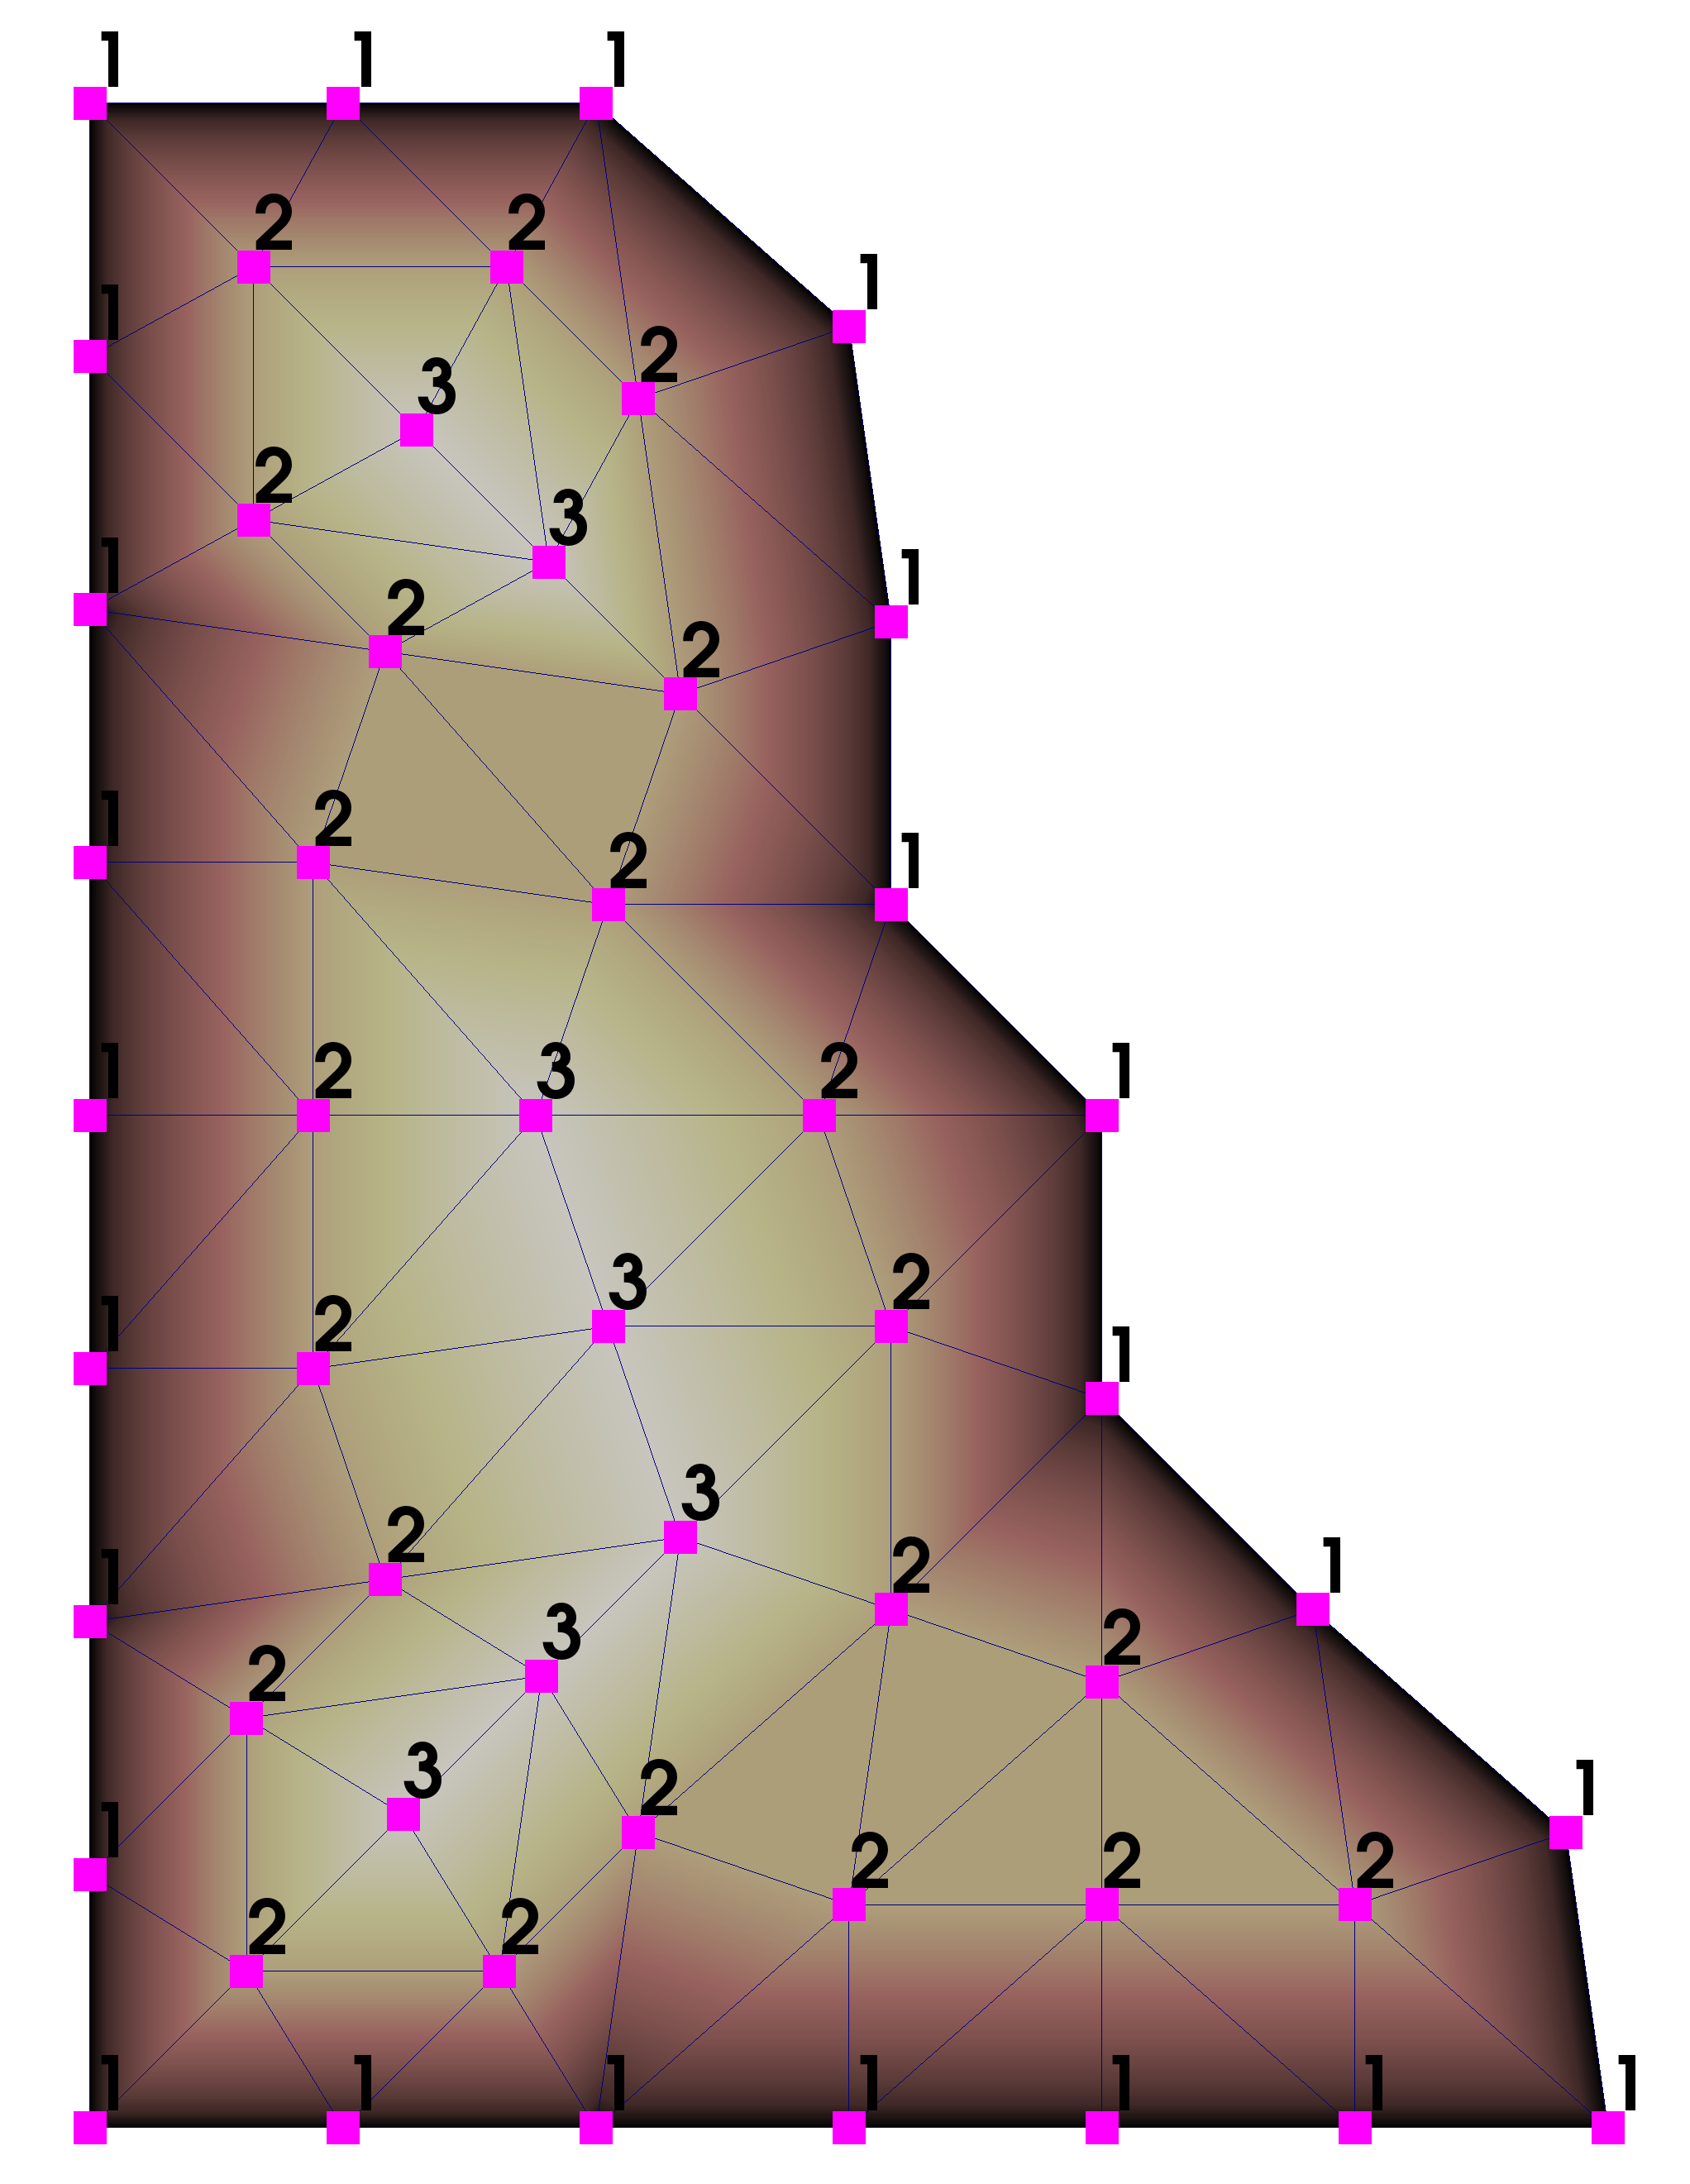
\includegraphics[width=.4\textwidth]{figures/2dTreeDepth.png}
    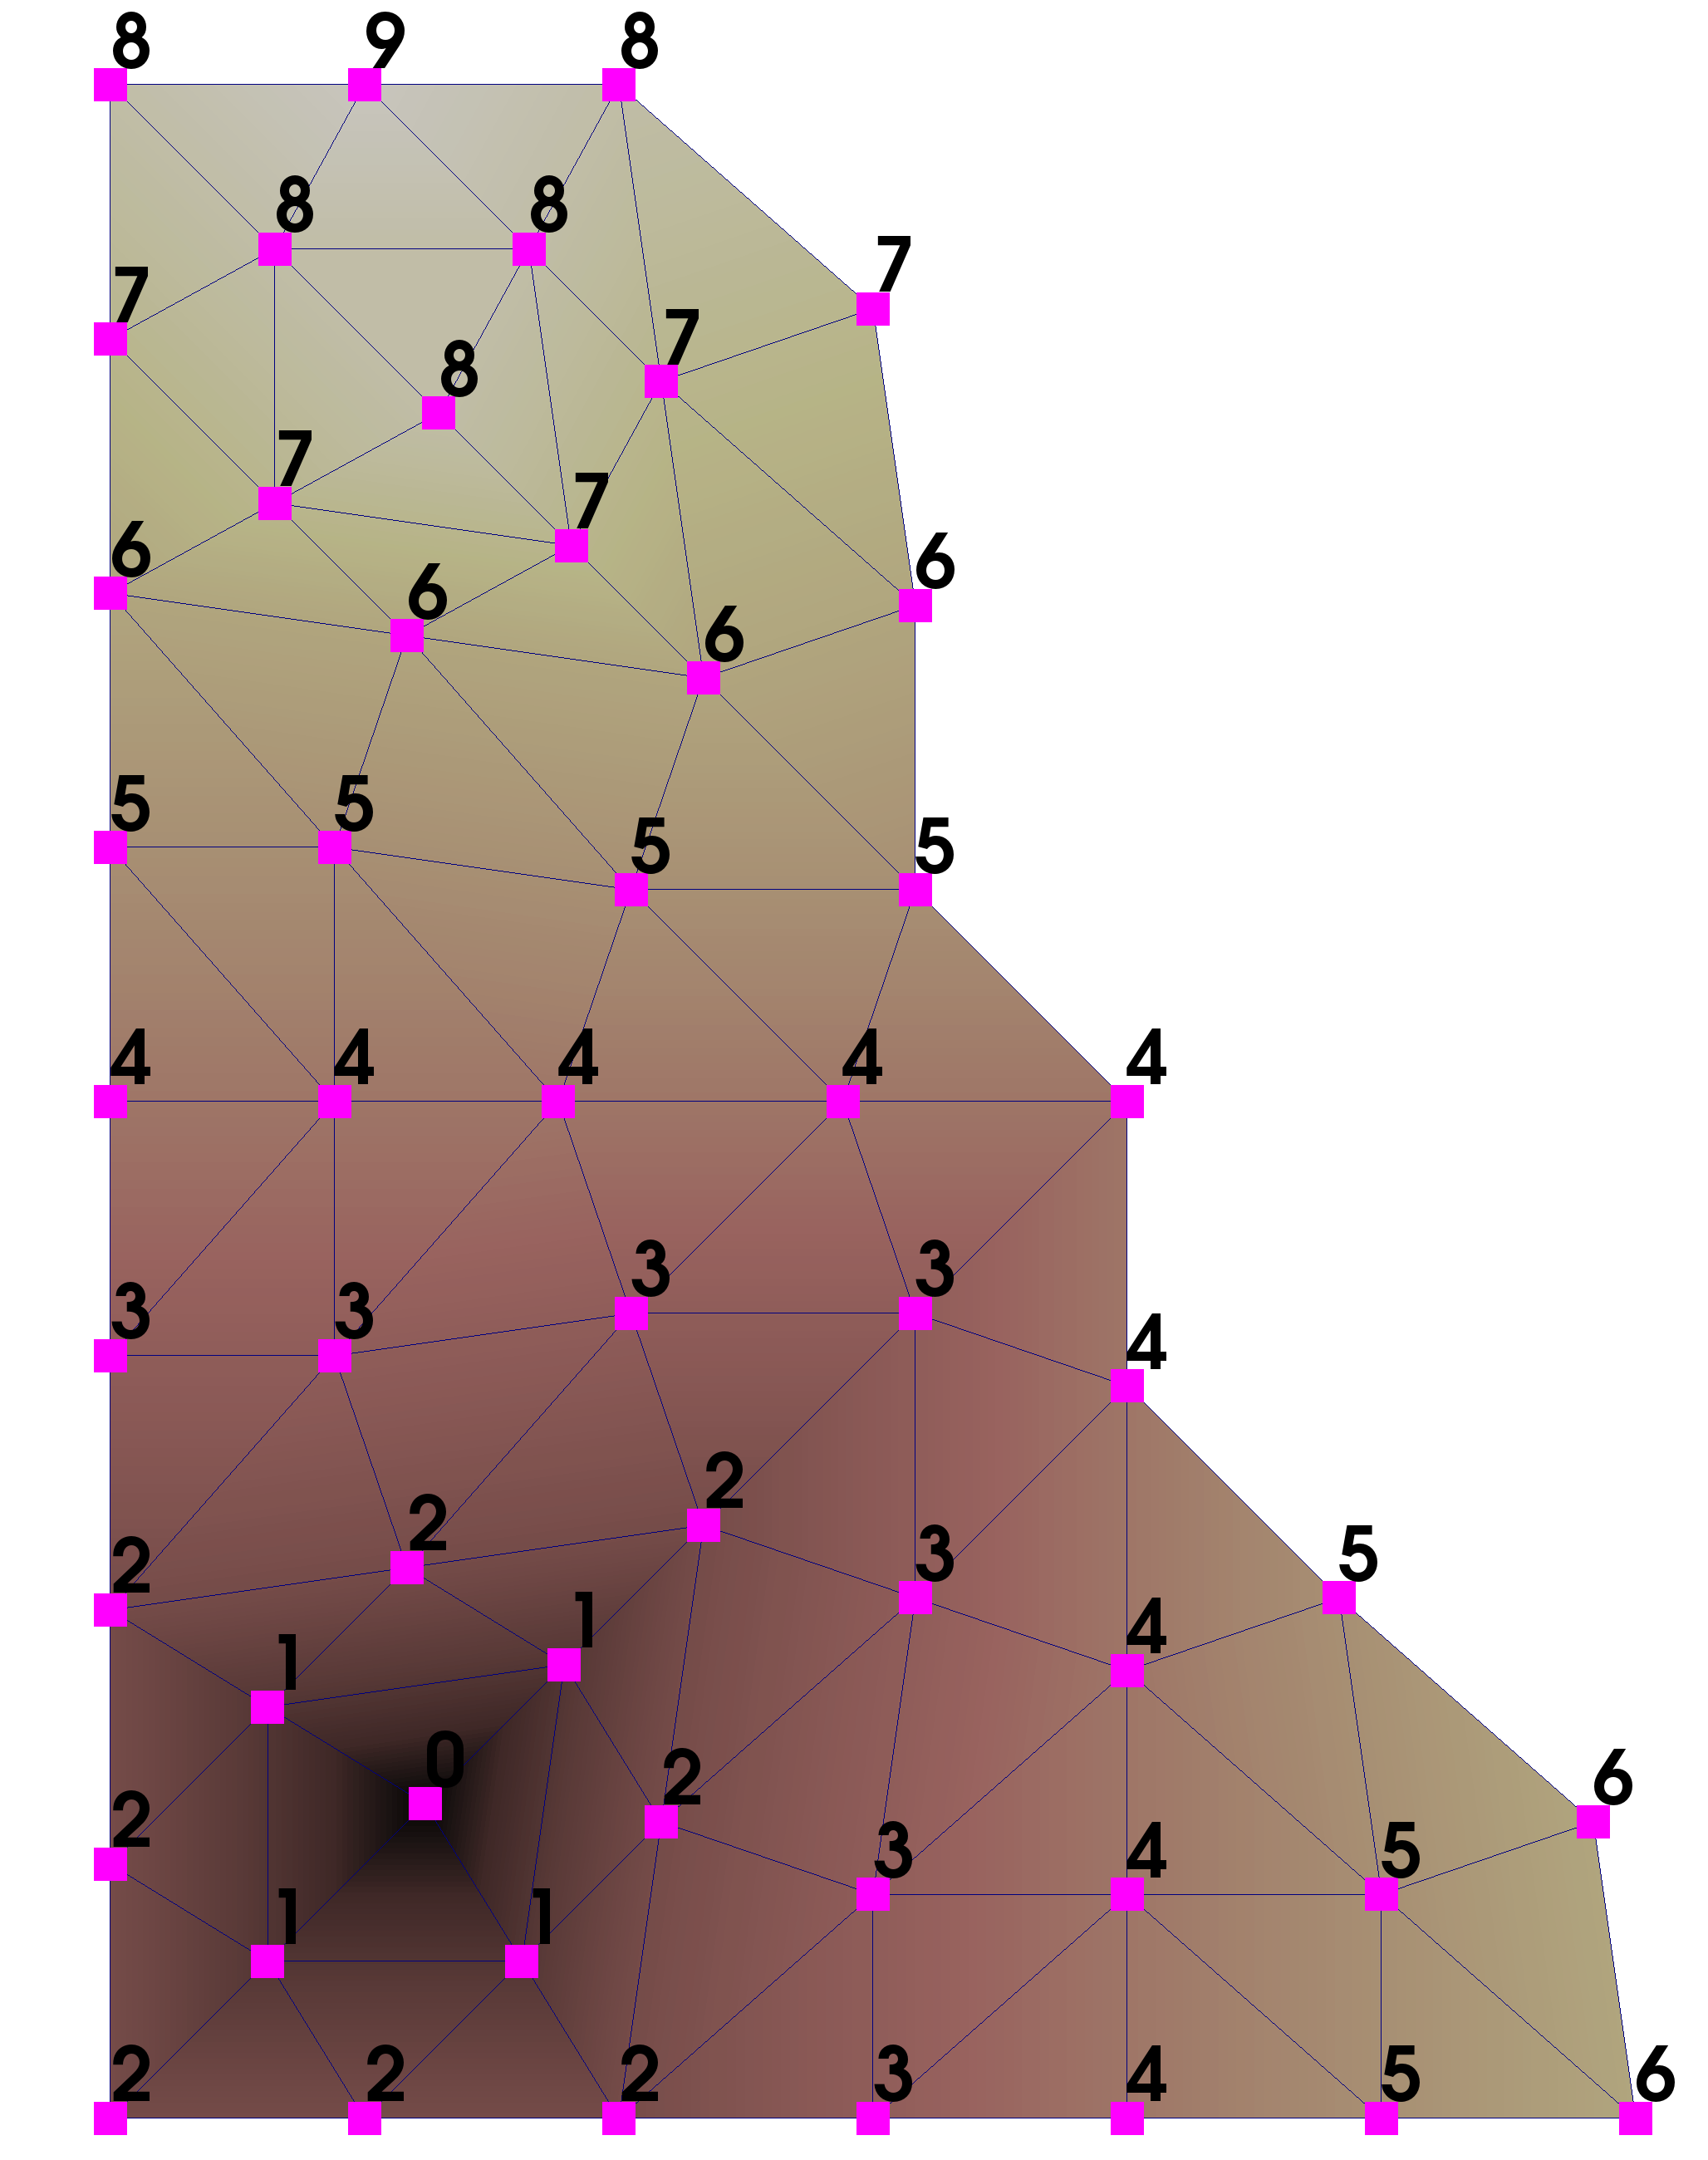
\includegraphics[width=.41\textwidth]{figures/2dDistance.png}
  \end{figure}
      (left) The distance from each vertex to the boundary and (right) the
    distance from the core vertex (marked with a zero near the
    bottom left corner).
\end{frame}

\begin{frame}
  \frametitle{Selection}
  \begin{minipage}{.5\textwidth}
    \begin{itemize}
    \item Iterates over (hyper)edges that cross a part boundary.
      
    \item The cavity defined by the (hyper)edge is chosen for migration if:
      \begin{itemize}
      \item The part that the (hyper)edge is shared with is a target part.
      \item The target part has not been sent more weight than the limit.
      \item The size of the cavity is small.
      \end{itemize}
    \end{itemize}
  \end{minipage}
  \begin{minipage}{.45\textwidth}

    \begin{figure}
      \centering
      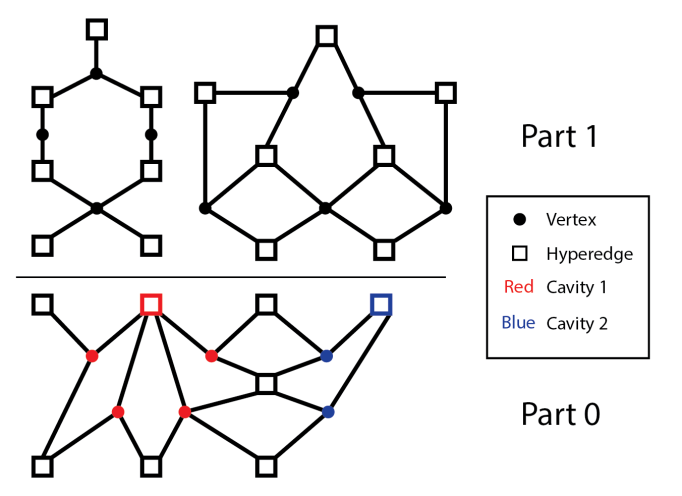
\includegraphics[width=\textwidth]{figures/PartBoundary.png}
    \end{figure}
  \end{minipage}
\end{frame}

\section{Partition Improvement Results}
\begin{frame}
  \frametitle{}
  \center \huge{Partition Improvement Results}
\end{frame}

\begin{frame}
  \frametitle{Problem Setup}
  We evaluate EnGPar's ability to improve vertex-centric
  and element-centric partitions created by ParMETIS.\\
  \medskip
  EnGPar is set to balance a mesh for a finite element and finite volume analysis where:
  \begin{itemize}
    \item Scalability of matrix formation is sensitive to secondary entity imbalance.
    \item Linear algebra routines are sensitive to the imbalance of degrees of freedom.
    \item Degrees of freedom are associated with primary entities.
  \end{itemize}
  \bigskip
  EnGPar first balances the DOF holders and then the secondary entity.
  target imbalance of 1.05. \\
  The imbalance of a given type (vtx, edge, face, or region) is defined as the 
  max part weight divided by the avg part weight.
\end{frame}

\begin{frame}
  \frametitle{Element Partition: Problem Setup}
  \medskip
  Element-centric tests were run on a billion element mesh. \\
  All experiments were run on the Mira BlueGene/Q system with one process per
  hardware thread. \\
  \smallskip
  Initial partitions are built using:
  \begin{itemize}
  \item Global ParMETIS part k-way to 8Ki($8*2^{10}$) parts.
  \item Local ParMETIS part k-way from 8Ki to 128Ki, 256Ki, and 512Ki parts.
  \end{itemize}
  The partitions before using EnGPar:\\
  \begin{table}[!h]
    \centering
    \begin{tabular}{||c|c|c|c||}
      \hline
      Number of Parts &128Ki&256Ki&512Ki \\
      \hline
      Elements per part & 9,836 & 4,918&2,459  \\
      \hline
      Vertex imbalance & 1.13 & 1.18 & 1.53 \\
      \hline
      Element imbalance & 1.02& 1.02& 1.02\\
      \hline
    \end{tabular}
  \end{table}
\end{frame}

\begin{frame}
  \frametitle{Element Partition: Mesh Vertex and Element Imbalance}
  \begin{figure}
    \centering
    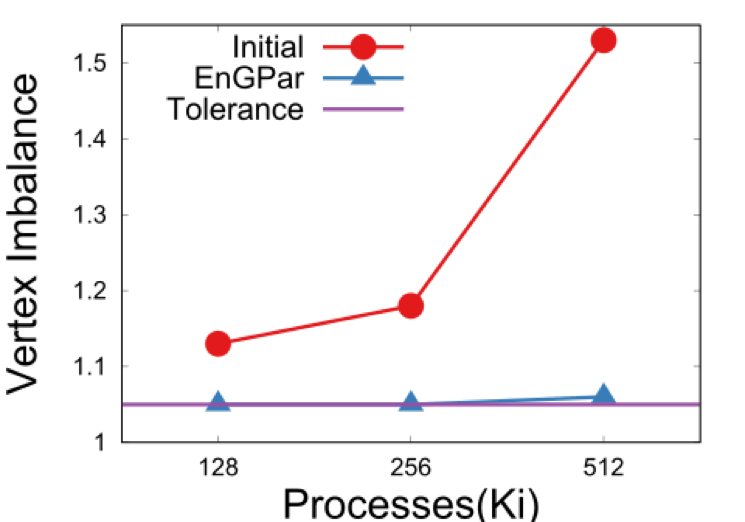
\includegraphics[width=.49\textwidth]{figures/elmPtn_vtxImb.png}
    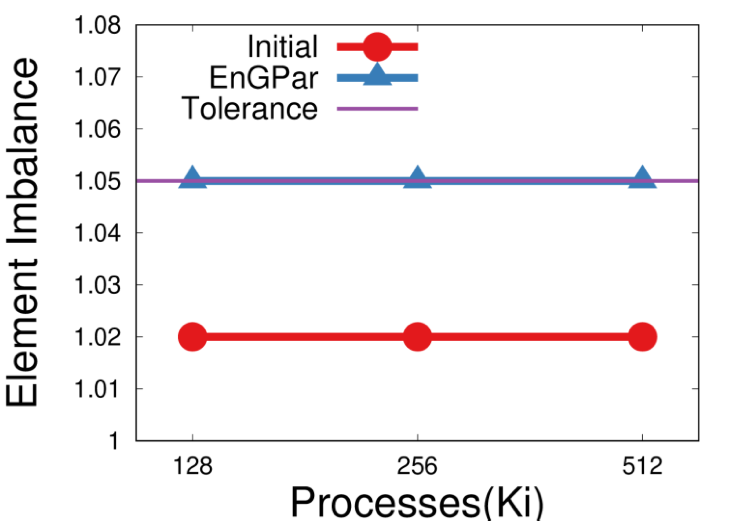
\includegraphics[width=.49\textwidth]{figures/elmPtn_elmImb.png} \\
    Mesh vertex imbalances is reduced from 13\% to 5\% for 128Ki, 18\% to 5\% for
    256Ki, and 53\% to 6\% for 512Ki.  Edge cut is increased by 1\%.
  \end{figure}  
\end{frame}

\begin{frame}
  \frametitle{Vertex Partition: Problem Setup}
  \medskip
  Vertex-centric tests were run on a 60 million element mesh. \\
  All experiments were run on the Mira BlueGene/Q system. \\
  \smallskip
  Initial partitions are built using:
  \begin{itemize}
  \item Global ParMETIS part k-way to 8Ki($8*2^{10}$) parts.
  \end{itemize}
  The partitions before using EnGPar: \\
  \begin{table}[!h]
    \centering
    \begin{tabular}{||c|c|c|c|c||}
      \hline
      Number of Parts   & 1Ki   & 2Ki   & 4Ki   & 8Ki \\
      \hline
      Vertices per part & 17,984 & 8,992 & 4,496 & 2,248 \\
      \hline
      Vertex imbalance  & 1.05  & 1.05  & 1.05  & 1.05 \\
      \hline
      Element imbalance & 1.99  & 2.0  & 1.99  & 2.00 \\
      \hline
    \end{tabular}
  \end{table}
  ParMETIS sacrifices element imbalance for a low edge cut.
\end{frame}

\begin{frame}
  \frametitle{Vertex Partition: Mesh Element Imbalance and Edge Cut}
  \begin{figure}
    \centering
    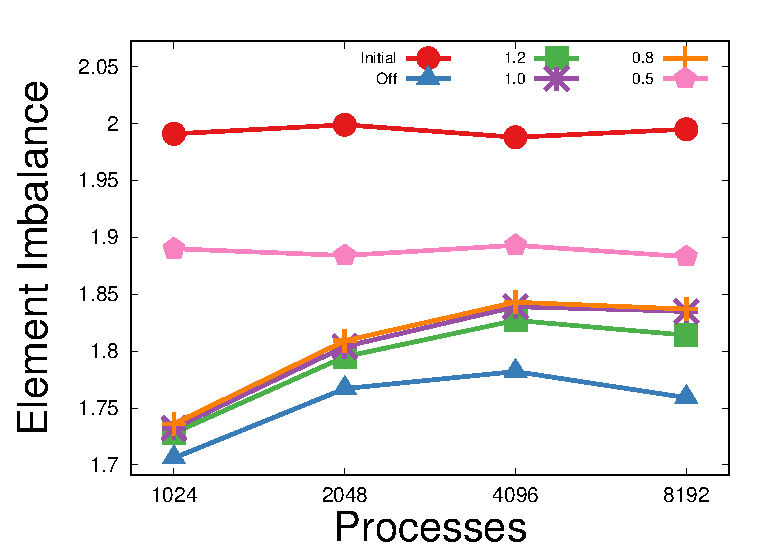
\includegraphics[width=.48\textwidth]{figures/eimb_v_cores.eps}
    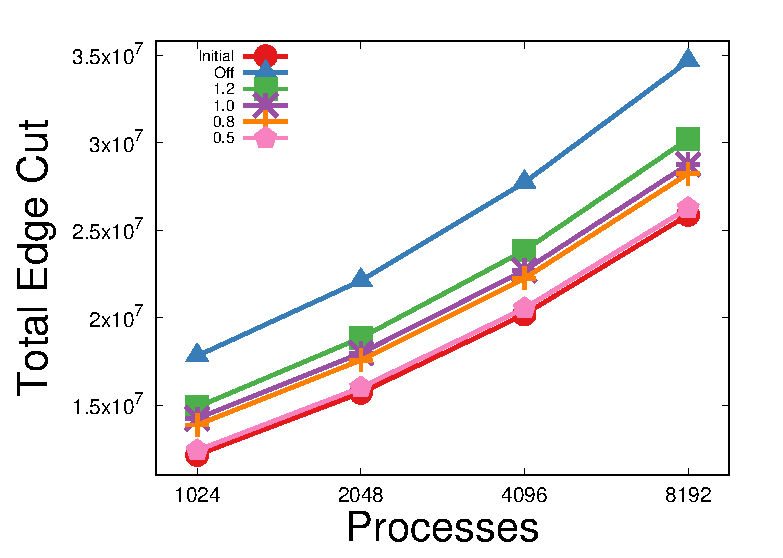
\includegraphics[width=.48\textwidth]{figures/ecut_v_cores.eps}\\
    Tuning the edge cut metric maintains the ParMETIS edge cut while reducing the
    edge imbalance by up to 5\%.
  \end{figure}  
\end{frame}

\section{Accelerating Selection Performance on GPUs}

\begin{frame}
  \frametitle{}
  \center \huge{Accelerating Selection Performance on GPUs}
\end{frame}

%\begin{frame}
%    \centering
%    \animategraphics[scale=0.5]{12}{figures/trap/boulder-}{0}{59}
%\end{frame}

\begin{frame}
  \frametitle{Where is time currently spent in EnGPar?}
  \begin{columns}
    \begin{column}{0.5\textwidth}
      Migration is 50\% of total time at 512Ki, 48\% at 256Ki, and 44\% at 128Ki
      \begin{itemize}
        \item General implementation sends/receives vertices and their adjacent
          (hyper)edges to/from any neighbor - communications on host
        \item Each process rebuilds its hypergraph after communications complete
      \end{itemize}
    \end{column}

    \begin{column}{0.5\textwidth}
      \begin{figure}
        \centering
        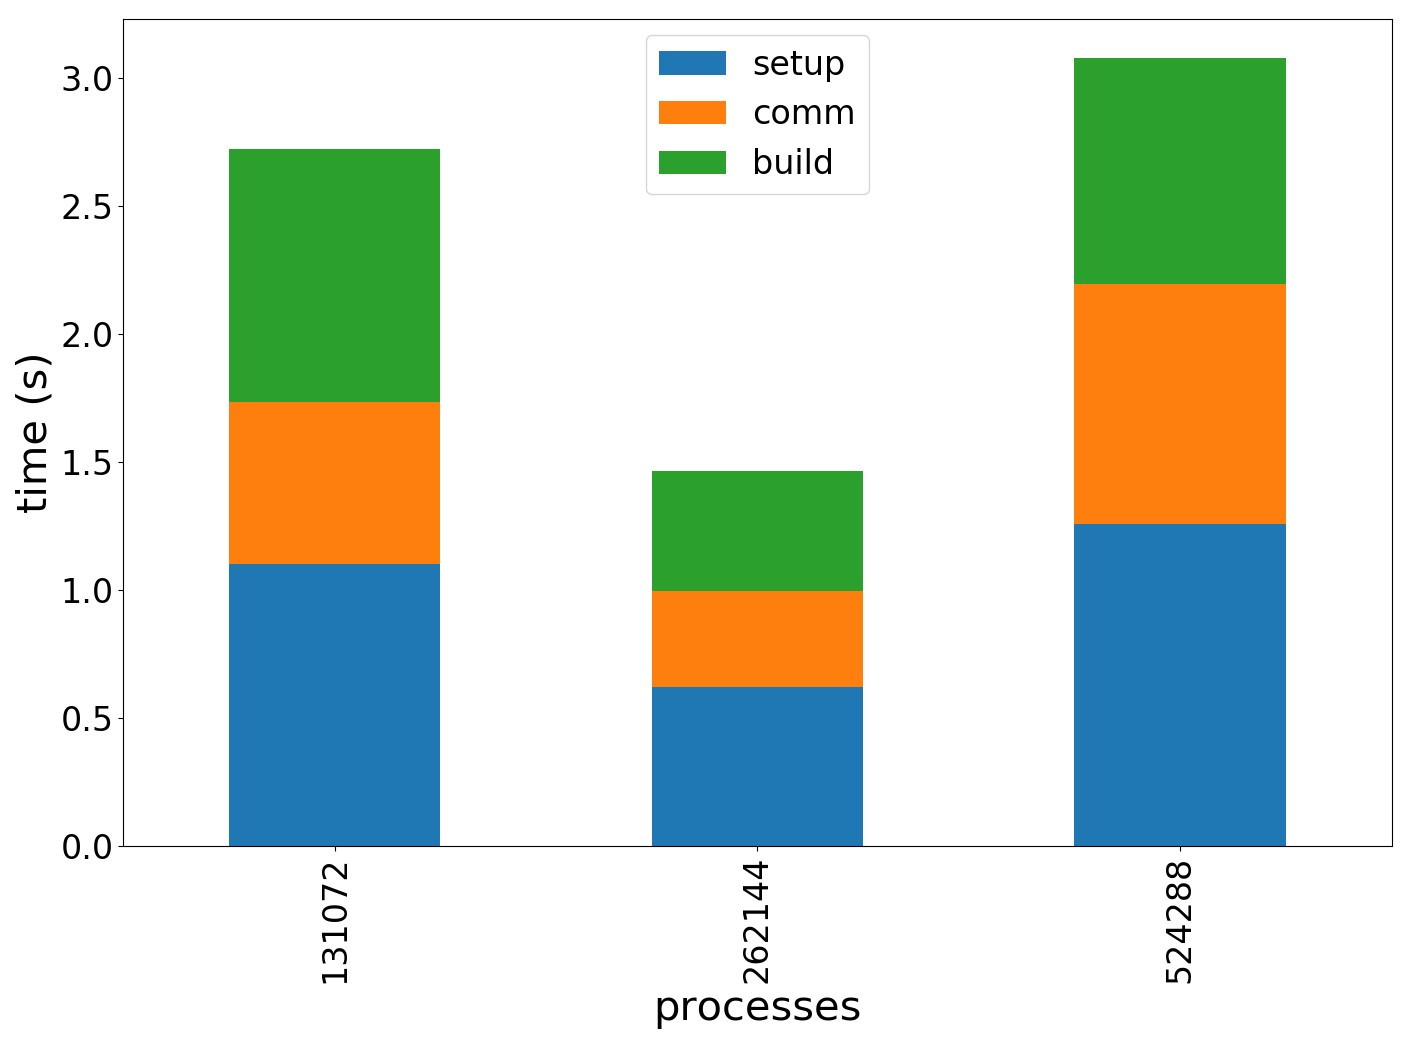
\includegraphics[width=.8\textwidth]{results/aero1Belm/migration.png}\\
        \tiny 1B elm mesh balanced on 128Ki, 256Ki, and 512Ki with EnGPar
      \end{figure}
    \end{column}
  \end{columns}
  \bigskip
  We want to improve the performance of these processes - that is a difficult
  task to start with.
  
  First let's see if we can accelerate something easier; selection of graph
  vertices to migrate.
\end{frame}

\begin{frame}
  \frametitle{BFS}
  Degree and diameter matters.
  \begin{itemize}
    \item Traversal of scale free graphs introduces additional
      complexities $\rightarrow$ specific algoritms to balance degree disparity.
    \item Traversal of low diameter graphs have larger frontiers and fewer
      synchronizations.
  \end{itemize}
  The selected method depends on architecture and graph characteristics
  \begin{itemize}
    \item Manycore - serial and shared memory parallel vertex-based, edge-based, push (vertices
      in the frontier push to next frontier), pull (all unvisited vertices check
      to for inclusion in next frontier)
    \item GPU - shared memory parallel versions of manycore procedures with data structure
      optimizations for coalesing, algebraic methods
  \end{itemize}
\end{frame}

\begin{frame}
  \frametitle{Our Approach}
  We will focus on hypergraphs created from unstructured meshes
  \begin{itemize}
    \item Downward adjacencies have uniform degree! ... not so much for upward
      adjacencies
    \item Diameter greatly depends on the geometric model and the
      partition - high quality parts are compact and have low diameter
  \end{itemize}
  Use Sell-C-Sigma datastructure for coalesing 
  \begin{itemize}
    \item Need weights for vertices and edges - lose some savings but retain
      improved vectorization
    \item Sorting (sigma) will be needed for meshes with semi-structured boundary layers (tet
      and wedge dominant with a handful of pyramids) and discrete event simulation graphs
  \end{itemize}
  Quantifying progress
  \begin{itemize}
    \item Time to solution, energy usage, GTEPS, and roofline analysis (TODO)
  \end{itemize}
\end{frame}

\begin{frame}
  \frametitle{Algorithms}
  The following variations of BFS were tested
  \begin{itemize}
    \item push - C++ serial push
    \item pull - C++ serial `pull' style vtx$\rightarrow$hyperedge
    \item csr - OpenCL parallel `pull' style vtx$\rightarrow$hyperedge using CSR data
      structure
    \item scg - OpenCL parallel `pull' style vtx$\rightarrow$hyperedge using
      Sell-C-Sigma data structure
    \item \texttt{*\_int} - use 4B int for adjacency and degree lists instead of 8B long
    \item \texttt{*\_unroll} - unroll the loop over hyperedges adjacent to a
      vertex
  \end{itemize}
  \begin{figure}
    \centering
    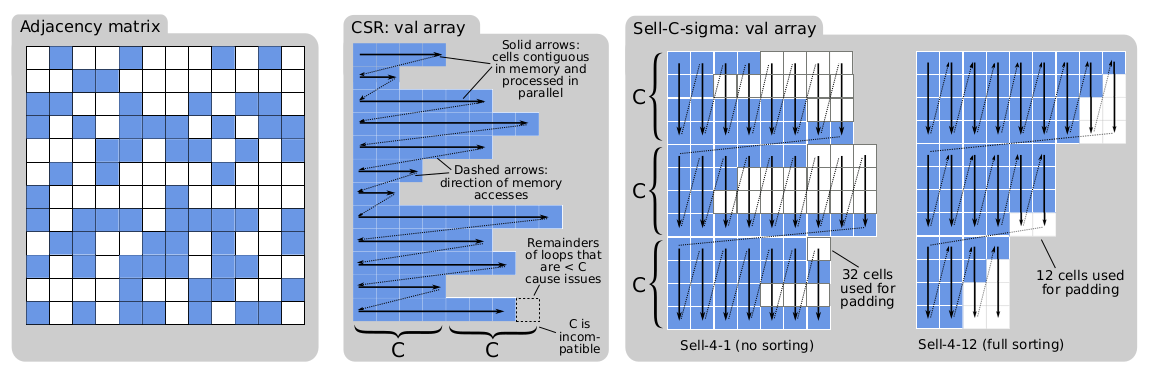
\includegraphics[width=.6\textwidth]{figures/sellcsigma.png}\\
    \small{Sell-C-Sigma data structure (Besta and Merending, et al.)}
  \end{figure}
\end{frame}

\begin{frame}
  \frametitle{Test Hypergraphs}
  Hypergraphs created from unstructured tet mesh of automotive part: \\
  mesh elements $\rightarrow$ graph vertices \\
  mesh vertices $\rightarrow$ hyperedges
  \begin{columns}

    \begin{column}{0.5\textwidth}
      \begin{figure}
        \centering
        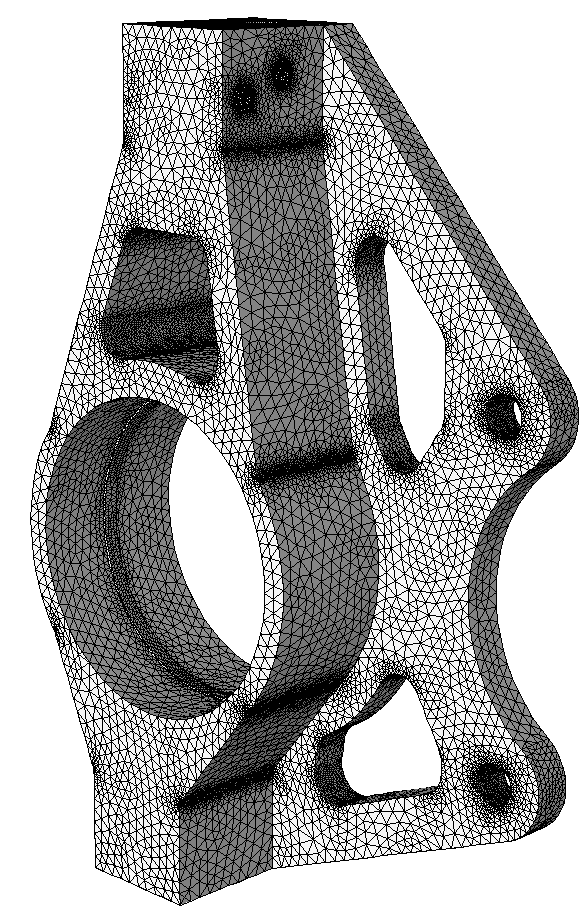
\includegraphics[width=.6\textwidth]{figures/upright400k.png}\\
        400k element mesh
      \end{figure}
    \end{column}

    \begin{column}{0.55\textwidth}
      \tiny
      \begin{table}[]
        \centering
        \begin{tabular}{lrrrr}
          graph & vertices & hyperedges & bfs levels & max frontier  \\
          67k   & 66433    & 15697      & 25         & 4432          \\
          190k  & 192728   & 40052      & 40         & 7992          \\
          400k  & 404613   & 88651      & 48         & 17316         \\
          890k  & 890925   & 187380     & 70         & 26664         \\
          1.6M  & 1580611  & 336215     & 82         & 45268         \\
          13M   & 12831104 & 2499193    & 82         & 95798         \\
          28M   & 27943315 & 5190006    & 210        &
        \end{tabular}\\
        \small{Hypergraphs}
      \end{table}
      \begin{figure}
        \vspace*{-.5cm}
        \centering
        \includegraphics[width=.85\textwidth]{results/frontsize/{scgopencl_chunk64_13M.frontsize}.png}
      \end{figure}
    \end{column}

  \end{columns}
\end{frame}

\begin{frame}
  \frametitle{BFS Results}
  Timing comparison of different OpenCL BFS kernels on NVIDIA 1080ti
  \begin{itemize}
    \item Includes data transfers, but not kernel JIT compilation; average of
      three runs shown
  \end{itemize}
  \texttt{scg\_int\_unroll} is 4.78 times faster than csr on 28M graph and up to 
      11 times faster than serial push on Intel Xeon (not shown) \\
  Memory coalescing is critical; \texttt{csr\_int\_unroll/scg\_int\_unroll} \\
  \begin{figure}
    \centering
    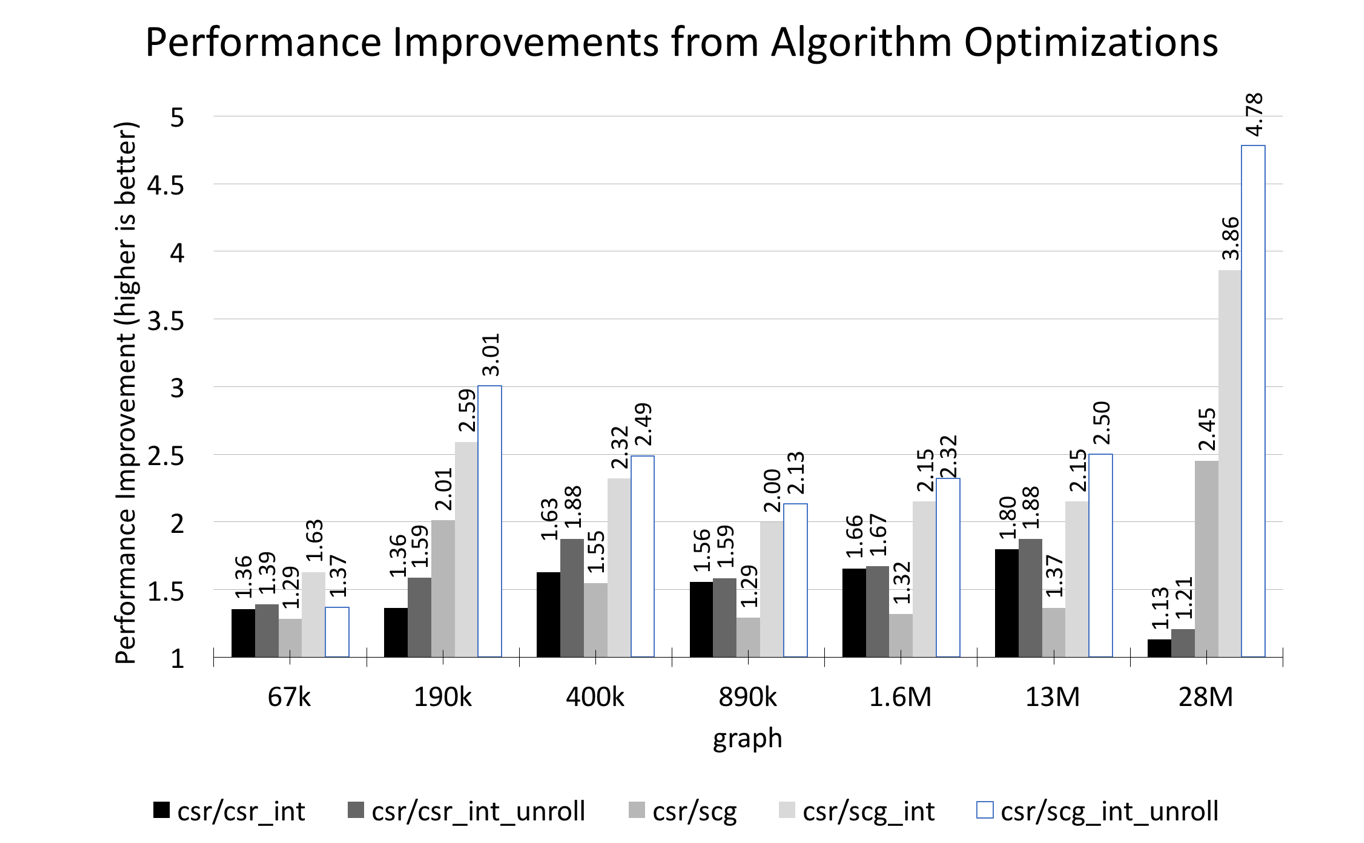
\includegraphics[width=.65\textwidth]{results/openclBfs.png}
  \end{figure}
\end{frame}

\begin{frame}
  \frametitle{Selection}
  Need to operate on non-overlapping cavities to avoid race condition - color the part boundary
  \begin{itemize}
    \item Coloring requires CSR of graph dual - hyperedges-to-hyperedges via vertices
    \item \texttt{Kokkos unordered\_map} - storing edge pairs \texttt{pair<int,int>}
  \end{itemize}
  A cavity is selected for migration if it satisfies color, target, and size criteria
  \begin{itemize}
    \item Each criteria is computed as a mask over the cavities
    \item $\land$ (logical and) the masks to select the cavities that meet all criteria
  \end{itemize}
  Challenge - managing duplicate adjacent entities e.g., second order adjacencies
 \end{frame}

\begin{frame}
  \frametitle{Parallel Coloring and Dual Computation}
  \begin{itemize}
    \item Speedup of parallel vs. serial on NVIDIA 1080ti
    \item Construction of dual is roughly constant
    \item Kokkos Coloring speedup increases with entity count - more parallelism
  \end{itemize}
  \begin{figure}
    \centering
    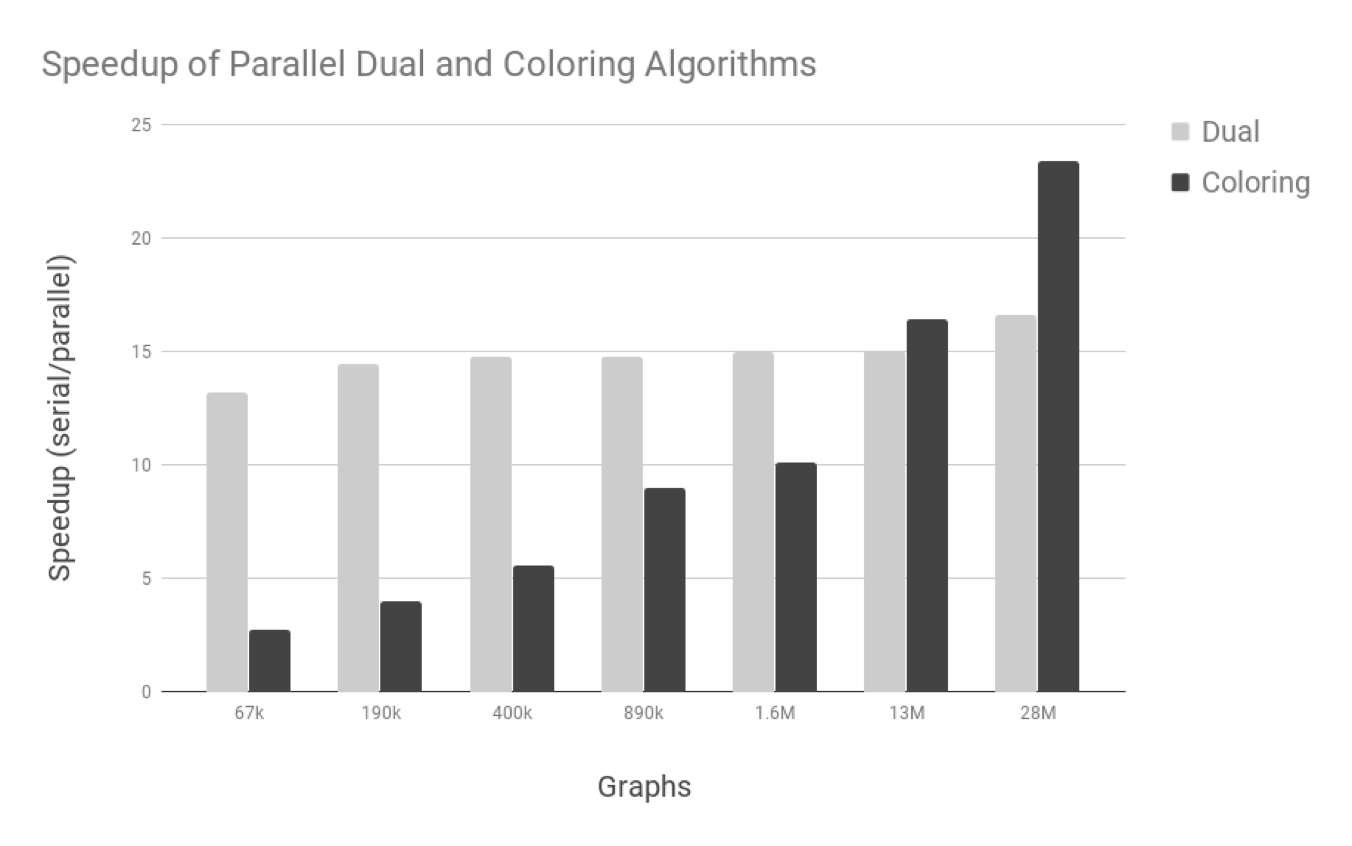
\includegraphics[width=.7\textwidth]{figures/kkColoringAndDual.png}
  \end{figure}
\end{frame}

\begin{frame}
  \frametitle{Parallel Selection}
  Almost there...
  \begin{figure}
    \centering
    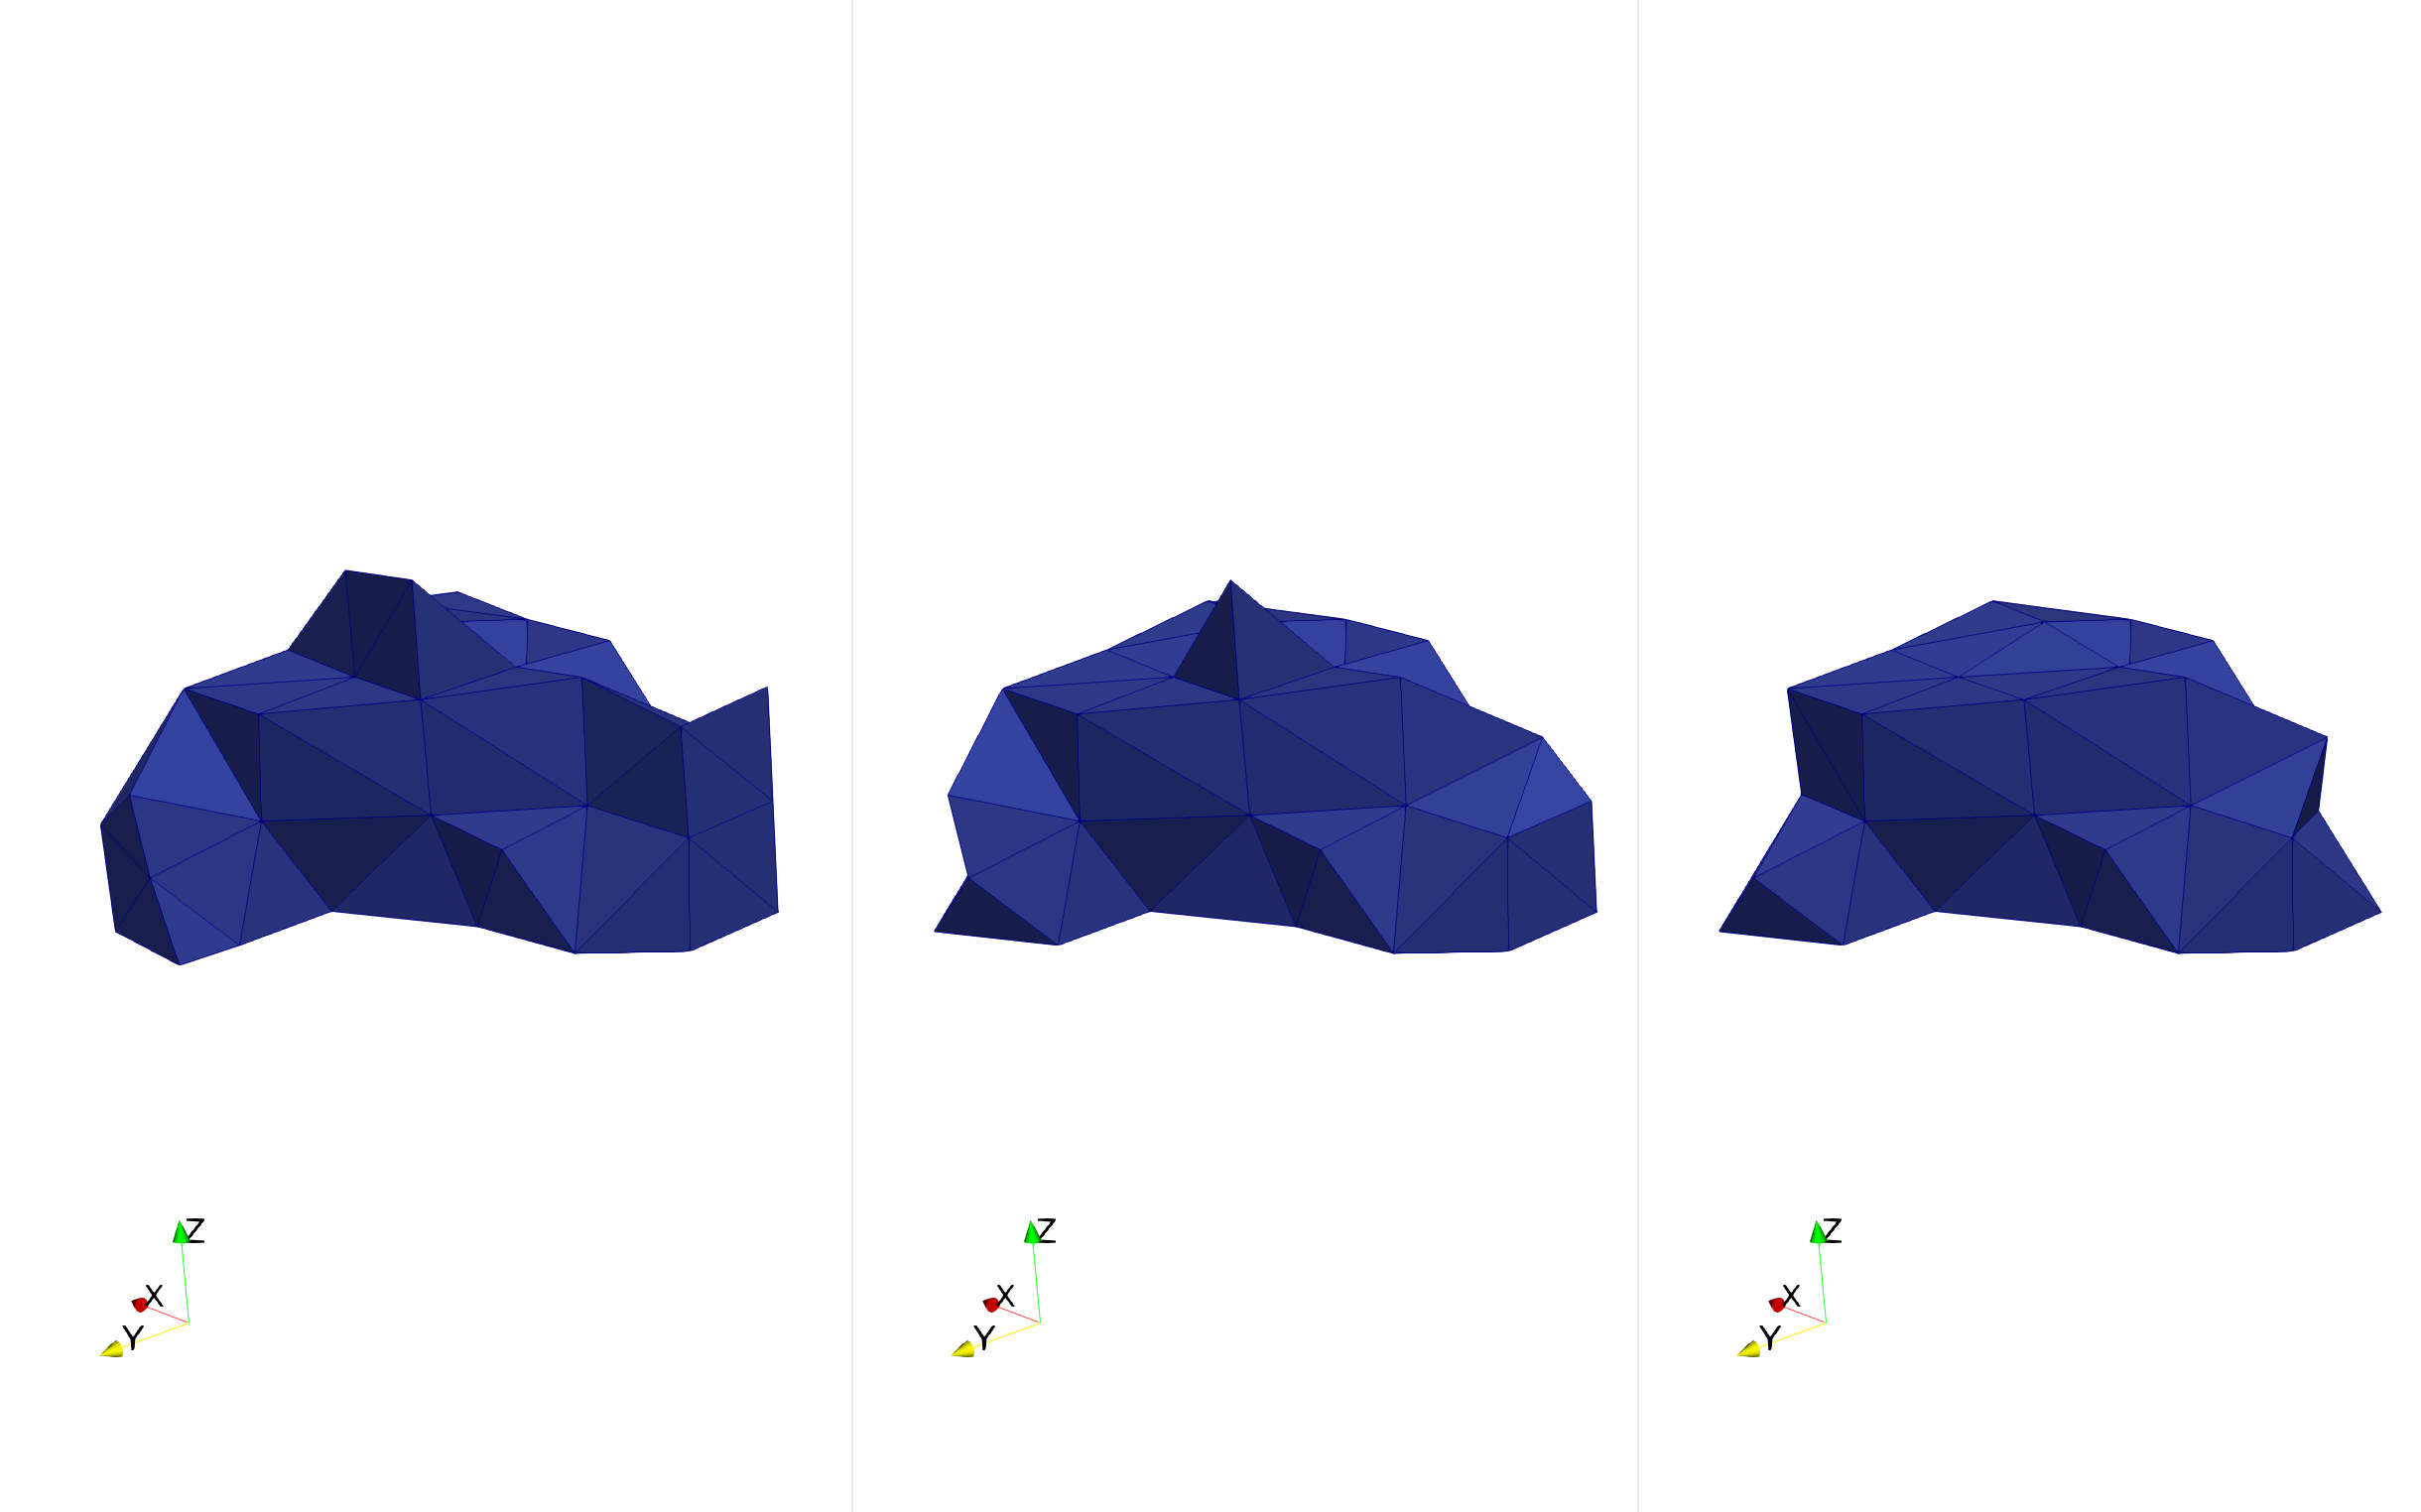
\includegraphics[width=\textwidth]{figures/selectionEx.png}
  \end{figure}
\end{frame}

\section{Accelerating Graph Operations on FPGAs}

\begin{frame}
  \frametitle{}
  \center \huge{Accelerating Graph Operations on FPGAs}
\end{frame}

\begin{frame}
  \frametitle{FPGA Architecture Review}
  \begin{columns}
    \begin{column}{0.5\textwidth}
      \begin{itemize}
        \item Reprogrammable device consisting of DSPs, multiply-accumulate blocks, hundreds of
          thousands of logic elements, registers, internal memory, external memory controllers, and an interconnect
        \item Multi TFLOPs per device, possible$^{*}$ to get near peak performance
        \item Programming: OpenCL, Xilinx Vivado HLS, OpenARC, initial OpenMP
        \item Long pipelines yield high performance
      \end{itemize}
    \end{column}
    \begin{column}{0.5\textwidth}
      \begin{figure}
        \centering
        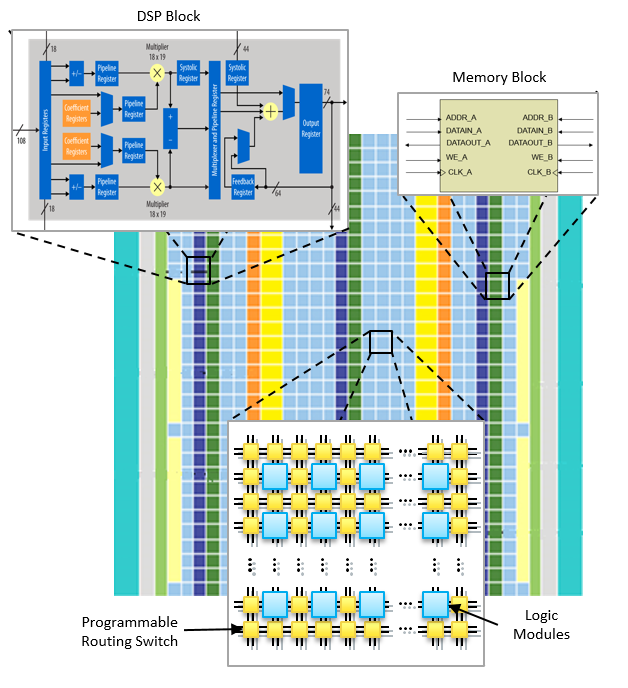
\includegraphics[width=\textwidth]{figures/fpga.png}
        {\tiny https://www.altera.com/documentation/}
      \end{figure}  
    \end{column}
  \end{columns}
\end{frame}

\begin{frame}
  \frametitle{FPGA: Pipelining Graph and Mesh Operations}
  \begin{columns}
    \begin{column}{0.65\textwidth}
      Different graph structures needed
      \begin{itemize}
        \item Static graph: breadth first search, reading stored adjacencies
        \item Dynamic graph: computing upward adjacencies, topology modifications (e.g., migration, adapt)
      \end{itemize}
      Example: graph inversion
      \begin{itemize}
        \item given a graph with uniform degree (e.g., downward adjacencies)
        \item add edge 0$\rightarrow$A to output graph if A$\rightarrow$0 exists in the input graph
        \item constructed graph has non-uniform degree
      \end{itemize}
    \end{column}
    \begin{column}{0.3\textwidth}
      \begin{figure}
        \centering
        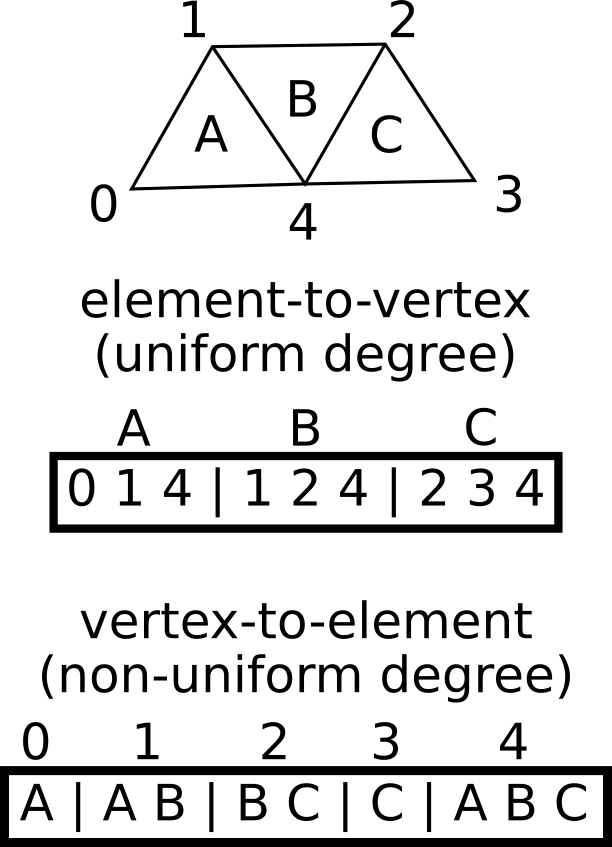
\includegraphics[width=.9\textwidth]{figures/exInvert.png}
      \end{figure}
    \end{column}
  \end{columns}
\end{frame}

\begin{frame}
  \frametitle{Our Circuit Using Vivado HLS}
  \begin{columns}
    \begin{column}{0.35\textwidth}
      Store the non-uniform graph as an array of shift registers
      \begin{itemize}
        \item all ops are pipelined with initialization interval of one cycle
        \item storing adjacencies (shift register) in BRAM reduces shift latency from 435 to 9 cycles
      \end{itemize}
    \end{column}
    \begin{column}{0.6\textwidth}
      \begin{figure}
        \centering
        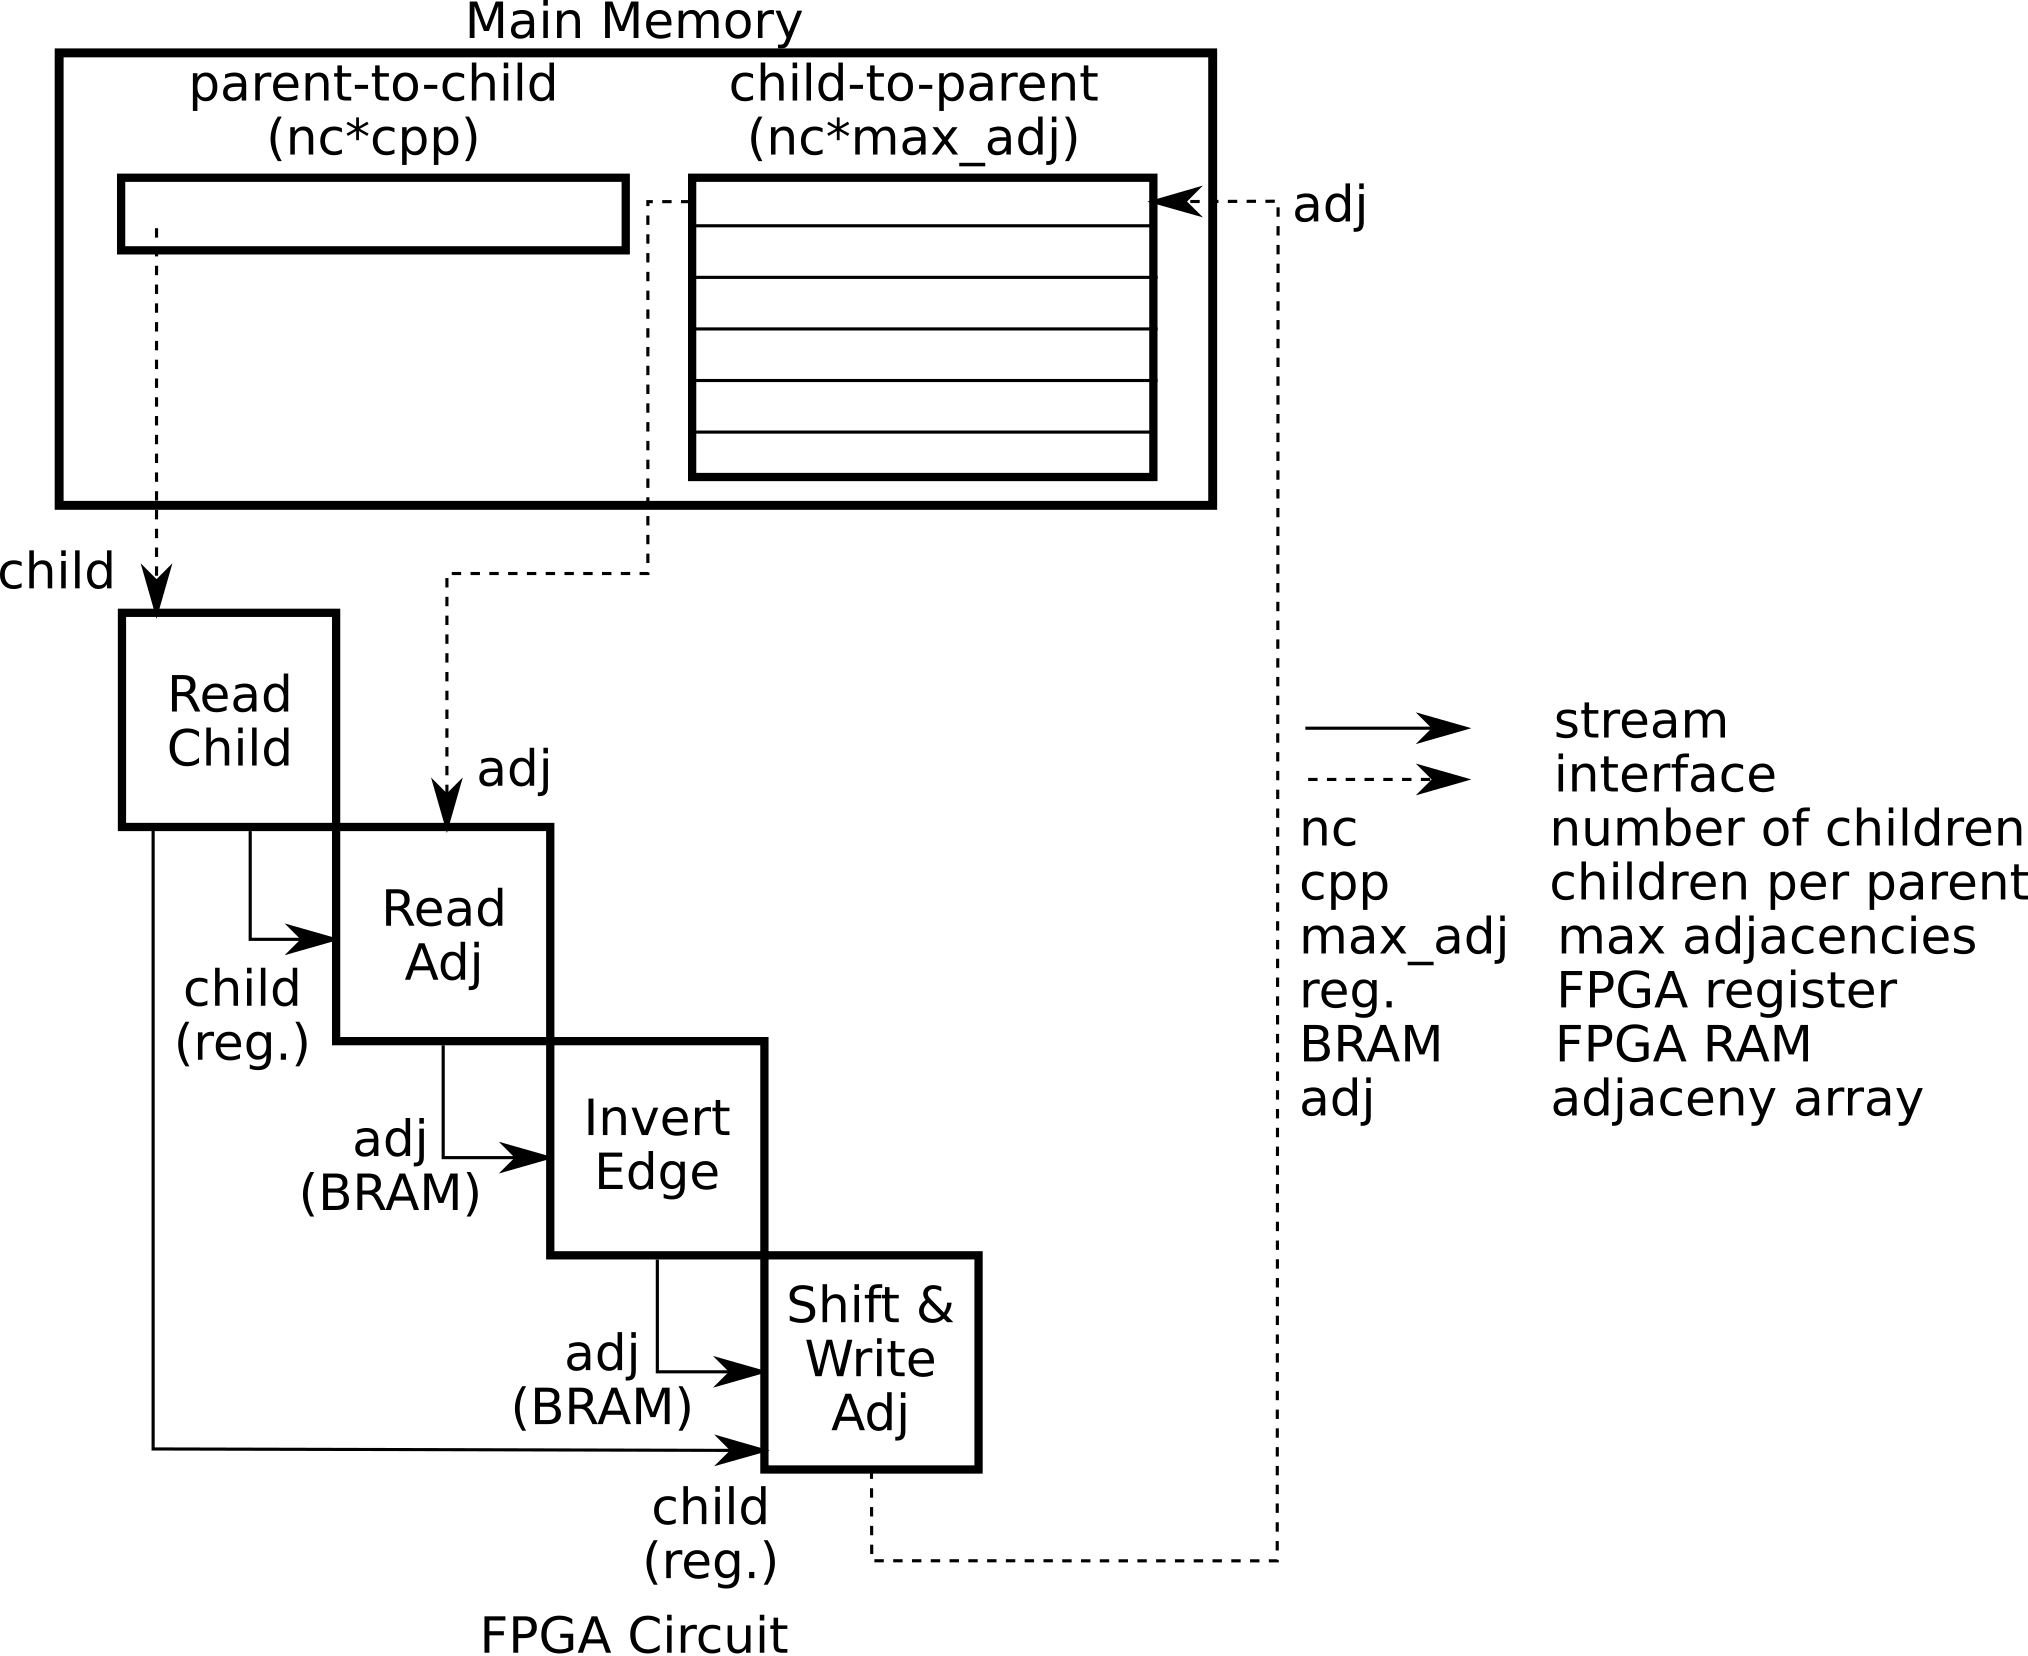
\includegraphics[width=\textwidth]{figures/invert.png}
      \end{figure}
      {\tiny "Initiation interval (II): Number of clock cycles before the function can accept new input data." - Xilinx Vivado HLS Users Guide}
    \end{column}
  \end{columns}
\end{frame}

\begin{frame}
  \frametitle{Closing Remarks}
  EnGPar:
  \begin {itemize}
  \item generalizing the diffusive load balancing algorithm developed in ParMA for applications without an element-based unstructured mesh.
  \item improving the algorithm of key portions to improve overall runtime.
  \end{itemize}
  MPI tests show that EnGPar:
  \begin {itemize}
  \item Reduces the high mesh vertex imbalance from the 512Ki mesh from 53\% to 6\%
  \item Maintains the mesh element imbalance at the tolerance.
  \end{itemize}
  Initial acceleration tests indicate:
  \begin {itemize}
  \item Utilizing known degree of downward adjacencies enables
    loop unrolling and improved load balance
  \item High performance FPGA graph processing circuits can be defined at the expense of additional memory
  \end{itemize}
\end{frame}

\begin{frame}
  \frametitle{Future Work}
  Expanding the capabilities of EnGPar:
  \begin{itemize}
    \item Continue improving partition quality when parts are small (i.e., strong scaling)
  \end{itemize}
  GPU Acceleration
  \begin{itemize}
    \item Porting BFS to Kokkos - add SCS, disconnected components
    \item Support migration - host communicates, device rebuilds (hyper)graph
    \item Test on bigger graphs
    \item Examine cost of second adjacencies
  \end{itemize}
  FPGA Pipelined Operations
  \begin{itemize}
    \item Sub-graph intersection and union, adjacency caching 
  \end{itemize}
  Applying EnGPar to other applications:
  \begin{itemize}
    \item XGCM - unstructured mesh based particle in cell plasma physics \url{epsi.pppl.gov/computing/xgc-1}
    \item FUN3D - a computational fluid dynamic simulation using a vertex-based partitioned mesh. \url{fun3d.larc.nasa.gov}
    \item PHASTA - massively parallel computational fluid dynamics. \url{github.com/PHASTA/phasta}
  \end{itemize}
\end{frame}

\begin{frame}
  \begin{center}
    {\huge
      Thank You\\
      \bigskip
      \bigskip
      \bigskip
      \bigskip
      \bigskip
      \huge
      Questions?\\
      \bigskip
      \bigskip
      \bigskip
    }
  \end{center}
  \large
  Acknowledgements:\\
  \begin{itemize}
    \item NSF SI2-SSE: Fast Dynamic Load Balancing Tools for Extreme Scale Systems
    \item DOE FASTMath SCIDAC Institute
    \item CEED ECP
    \item Argonne National Laboratory - Kazutomo Yoshii
    \item Xilinx University Program - access to hardware
  \end{itemize}
\end{frame}

\begin{frame}
  \center \huge Extra Slides
\end{frame}

\begin{frame}
  \frametitle{N-graph}
  The N-graph is a multigraph with two modes of operation: traditional or hypergraph.\\
  \smallskip
  The N-graph is defined as the following:
  \begin{itemize}
  \item A set of vertices $V$ representing the atomic units of work.
  \item If using the traditional graph mode:
    \begin{itemize}
    \item $N$ sets of edges $E_0,...,E_{n-1}$ for each type of relation.
    \item Each edge connects two vertices $u,v \in V$.
    \end{itemize}
  \item If using the hypergraph mode:
    \begin{itemize}
    \item $N$ sets of hyperedges $H_0,...,H_{n-1}$ for each type of relation.
    \item $N$ sets of pins $P_0,...,P_{n-1}$ corresponding to each set of hyperedges.
    \item Each pin in $P_i$ connects a vertex, $v \in V$, to a hyperedge $h \in H_i$.
    \end{itemize}
  \end{itemize}
\end{frame}

\begin{frame}
  \frametitle{Mapping example}
  %Figure showing the conversion from mesh to N-graph
  \begin{figure}
    \centering
    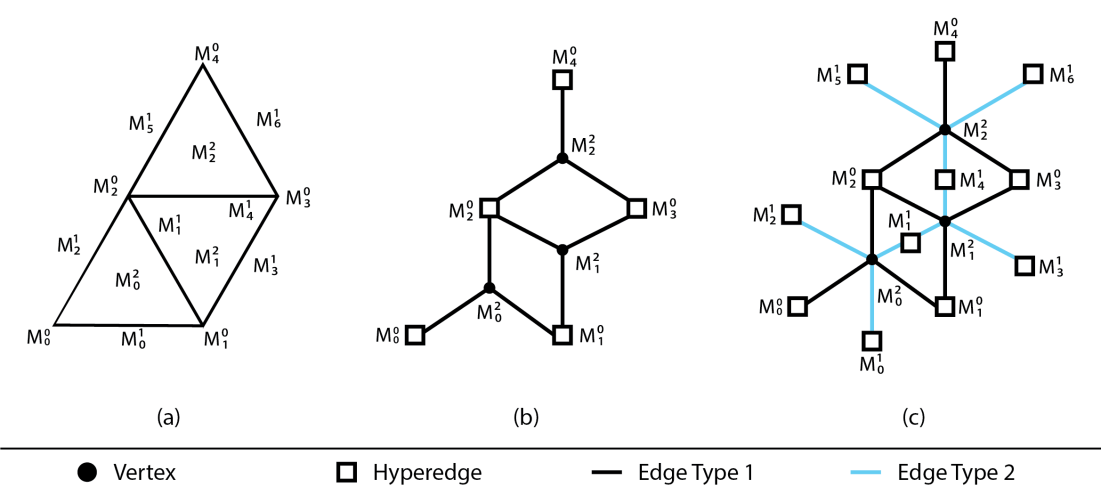
\includegraphics[width=.9\textwidth]{figures/exampleMesh2Graph.png}
    \caption{Converting a triangular mesh(a) to the N-graph with an edge type for mesh vertices (b) and an additional edge type for mesh edges (c).}
  \end{figure}
\end{frame}

\begin{frame}
  \frametitle{Diffusive Terminology}
  \begin{minipage}{0.45\textwidth}
  \begin{itemize}
  \item Sides
    \begin{itemize}
    \item Each part determines which parts are its neighbors.
    \item Determines a measurement of the area between each part.
    \end{itemize}
  \item Cavity
    \begin{itemize}
    \item Defined by (hyper)edges that cross a part boundary.
    \item Includes all the vertices that bound the (hyper)edge.
    \end{itemize}
  \end{itemize}
  \end{minipage} \hfill
  \begin{minipage}{0.5\textwidth}
  \begin{figure}
    \centering
    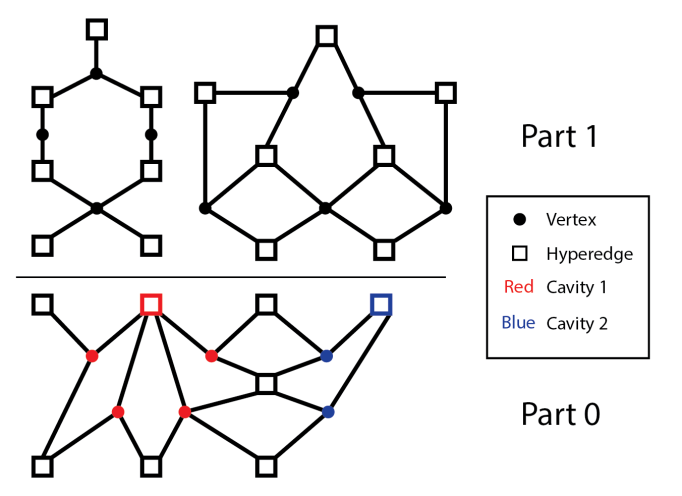
\includegraphics[width=\textwidth]{figures/PartBoundary.png}
    \caption{Two parts of an N-graph with a side of size 4. Two cavities are shown in red and blue for part 0.}
  \end{figure}
  \end{minipage}
\end{frame}

\begin{frame}
  \frametitle{Diffusive Terminology}
  \begin{itemize}
  \item Weights
    \begin{itemize}
    \item Each part computes its weight of the current target entity types, $w_i$.
    \item This weight is shared with all of the part's neighbors(sides).
    \end{itemize}
  \item Targets
    \begin{itemize}
    \item The neighbors that the part will send weight to.
    \item A part, $i$, will send weight to a neighbor, $j$, if:
      \begin{itemize}
      \item $w_i>w_j$
      \item the area between the parts ($s_{ij}$) is less than the average of all part boundaries.  
      \end{itemize}
    \item Weight to send from part $i$ to part $j$ is $\alpha(w_i-w_j)*\dfrac{\text{size}(s_{ij})}{\text{size}(s)}$
      \begin{itemize}
        \item $\alpha$ is an input parameter that limits how much weight is sent in each iteration.
      \end{itemize}
    \end{itemize}
  \end{itemize}
\end{frame}

\begin{frame}
  \frametitle{Architecture Review}
  Manycore
  \begin{itemize}
    \item Tens of out-of-order cores with hardware level pipelining
    \item 1-2 TFLOPs per processor/socket, possible$^{*}$ to get near
      peak
    \item Programming models and languages: shared memory,
      distributed, SHMEM, OpenMP, PThreads, MPI, etc.
    \item Efficient use of available memory bandwidth often yields peak performance - 
      supported by both data parallel and message passing models
  \end{itemize}
  GPU
  \begin{itemize}
    \item Many small cores organized into groups that run in lock-step
    \item Multi TFLOPs per device, hard to get near peak
    \item Programming models and languages: OpenMP, CUDA, OpenCL,
      OpenACC
    \item Wide data parallelism yields maximum performance - requires memory
      coalescing and minimal divergence
  \end{itemize}
\end{frame}


\begin{frame}
  \frametitle{Related Work on Accelerated BFS}
  Lots of it - mostly focused on scale-free graphs and using many-core
  and GPUs
  \begin{itemize}
    \item SlimSell - custom data structure for algebraic BFS (Hoefler)
    \item Global and Local Manhattan Collapse - inner/frontier loop transformations to
      improve load balance and reduce irregular memory access (Slota)
    \item Merijn - runtime switching of graph structure and push/pull algorithm based
      on front size and other factors (M. Verstraaten)
      % Merijn ---> Meer-hang
      % https://arxiv.org/pdf/1708.01159.pdf
      % https://github.com/merijn/GPU-benchmarks
% george's BFS references 
%% [3] - S. Beamer, K. Asanovic, and D. Patterson, “Direction- ´
%      optimizing breadth-first search,” in Proc. Int’l. Conf. for High
%      Performance Computing, Networking, Storage and Analysis
%      (SC), 2013.
%% [7] F. Checconi and F. Petrini, “Traversing trillions of edges
%      in real-time: Graph exploration on large-scale parallel machines,”
%      in Proc. IEEE Int’l. Parallel and Distributed Proc.
%      Symp. (IPDPS), 2014.
%% [12] T. Gao, Y. Lu, B. Zhang, and G. Suo, “Using the Intel
%      Many Integrated Core to accelerate graph traversal,” Sage
%      Int’l. Journal of High Performance Computing Applications,
%      vol. 28, no. 3, pp. 255–266, 2014.
%% [16] S. Hong, S. K. Kim, T. Oguntebi, and K. Olukotun, “Accelerating
%      CUDA graph algorithms at maximum warp,” in Proc.
%      ACM SIGPLAN Symp. on Principles and Practice of Parallel
%      Programming (PPoPP), 2011
%% [17] S. Hong, T. Oguntebi, and K. Olukotun, “Efficient parallel
%      graph exploration on multi-core CPU and GPU,” in Proc.
%      Int’l. Conf. on Parallel Architectures and Compilation Techniques
%      (PACT), 2011.
%% [23] D. Merrill, M. Garland, and A. Grimshaw, “Scalable GPU
%      graph traversal,” in Proc. ACM SIGPLAN Symp. on Principles
%      and Practice of Parallel Programming (PPoPP), 2012.
  \end{itemize}
  Can we apply some of these approaches to a hyper multi-graph and run
  effectively on manycore CPUs, GPUs, and FPGAs?
\end{frame}


\begin{frame}
  \frametitle{Other View of Results}
  \tiny
  Timing comparison of different kernels on NVIDIA 1080ti - includes sequential
  push
  \begin{itemize}
    \item Includes data transfers, but not kernel JIT compilation
    \item The average of three runs is used for the comparison
    \item Higher is better
  \end{itemize}
  \begin{figure}
    \centering
    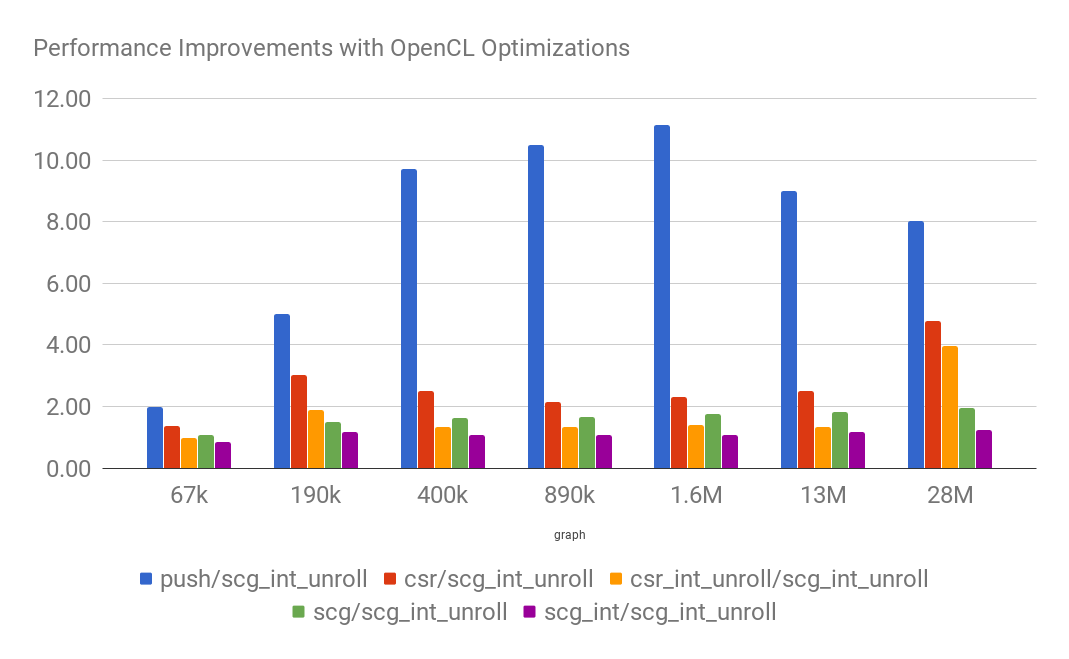
\includegraphics[width=.9\textwidth]{results/bfs.png}
  \end{figure}  
\end{frame}

\begin{frame}
  \frametitle{Gripes}
  OpenCL 
  \begin{itemize}
    \item Isn't supported on Power9+V100 deployments yet - can't build kernels
    \item OCLgrind was the only useful debugging tool I could find (github.com/jrprice/Oclgrind)
    \item Shiny (not so) new language features (e.g., team collectives) are not supported by devices I tested on
  \end{itemize}
  FPGAs
  \begin{itemize}
    \item 5hr+ compile time
    \item steep learning curve for development
  \end{itemize}
\end{frame}

\begin{frame}
  \frametitle{Example of N-Graph CSR}
  Our current N-Graph data structure is two sets of compressed sparse row (CSR)
  structures
  \begin{figure}
    \centering
    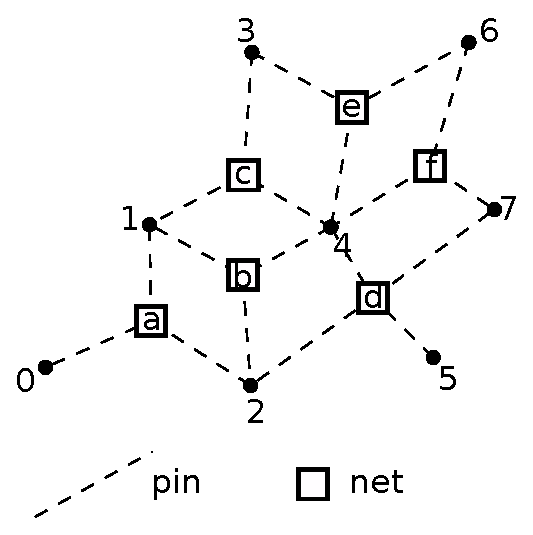
\includegraphics[width=.4\textwidth]{figures/hypergraph.eps}
  \end{figure}  
  {\tiny
  \begin{table}[]
    \centering
    \label{my-label}
    \begin{tabular}{llllllllll}
      vtx id                 & 0     & 1     & 2     & 3       & 4         & 5     & 6   & 7   &    \\
      vtx-to-net offsets     & 0     & 1     & 4     & 7       & 9         & 14    & 15  & 17  & 19 \\
      vtx-to-net adjacencies & a     & a,b,c & a,b,d & c,e     & b,c,d,e,f & d     & e,f & d,f &    \\
      \hline
      net id                 & a     & b     & c     & d       & e         & f     &     &     &    \\
      net-to-vtx offsets     & 0     & 3     & 5     & 8       & 12        & 15    & 18  &     &    \\
      net-to-vtx adjacencies & 0,1,2 & 1,2   & 1,3,4 & 2,4,5,7 & 3,4,6     & 4,6,7 &     &     &   
    \end{tabular}
  \end{table}
  }
\end{frame}

\begin{frame}{BFS SCG Kernel and Loop}
  \begin{columns}
    \begin{column}{0.5\textwidth}
      Kernel:
      \begin{figure}
        \centering
        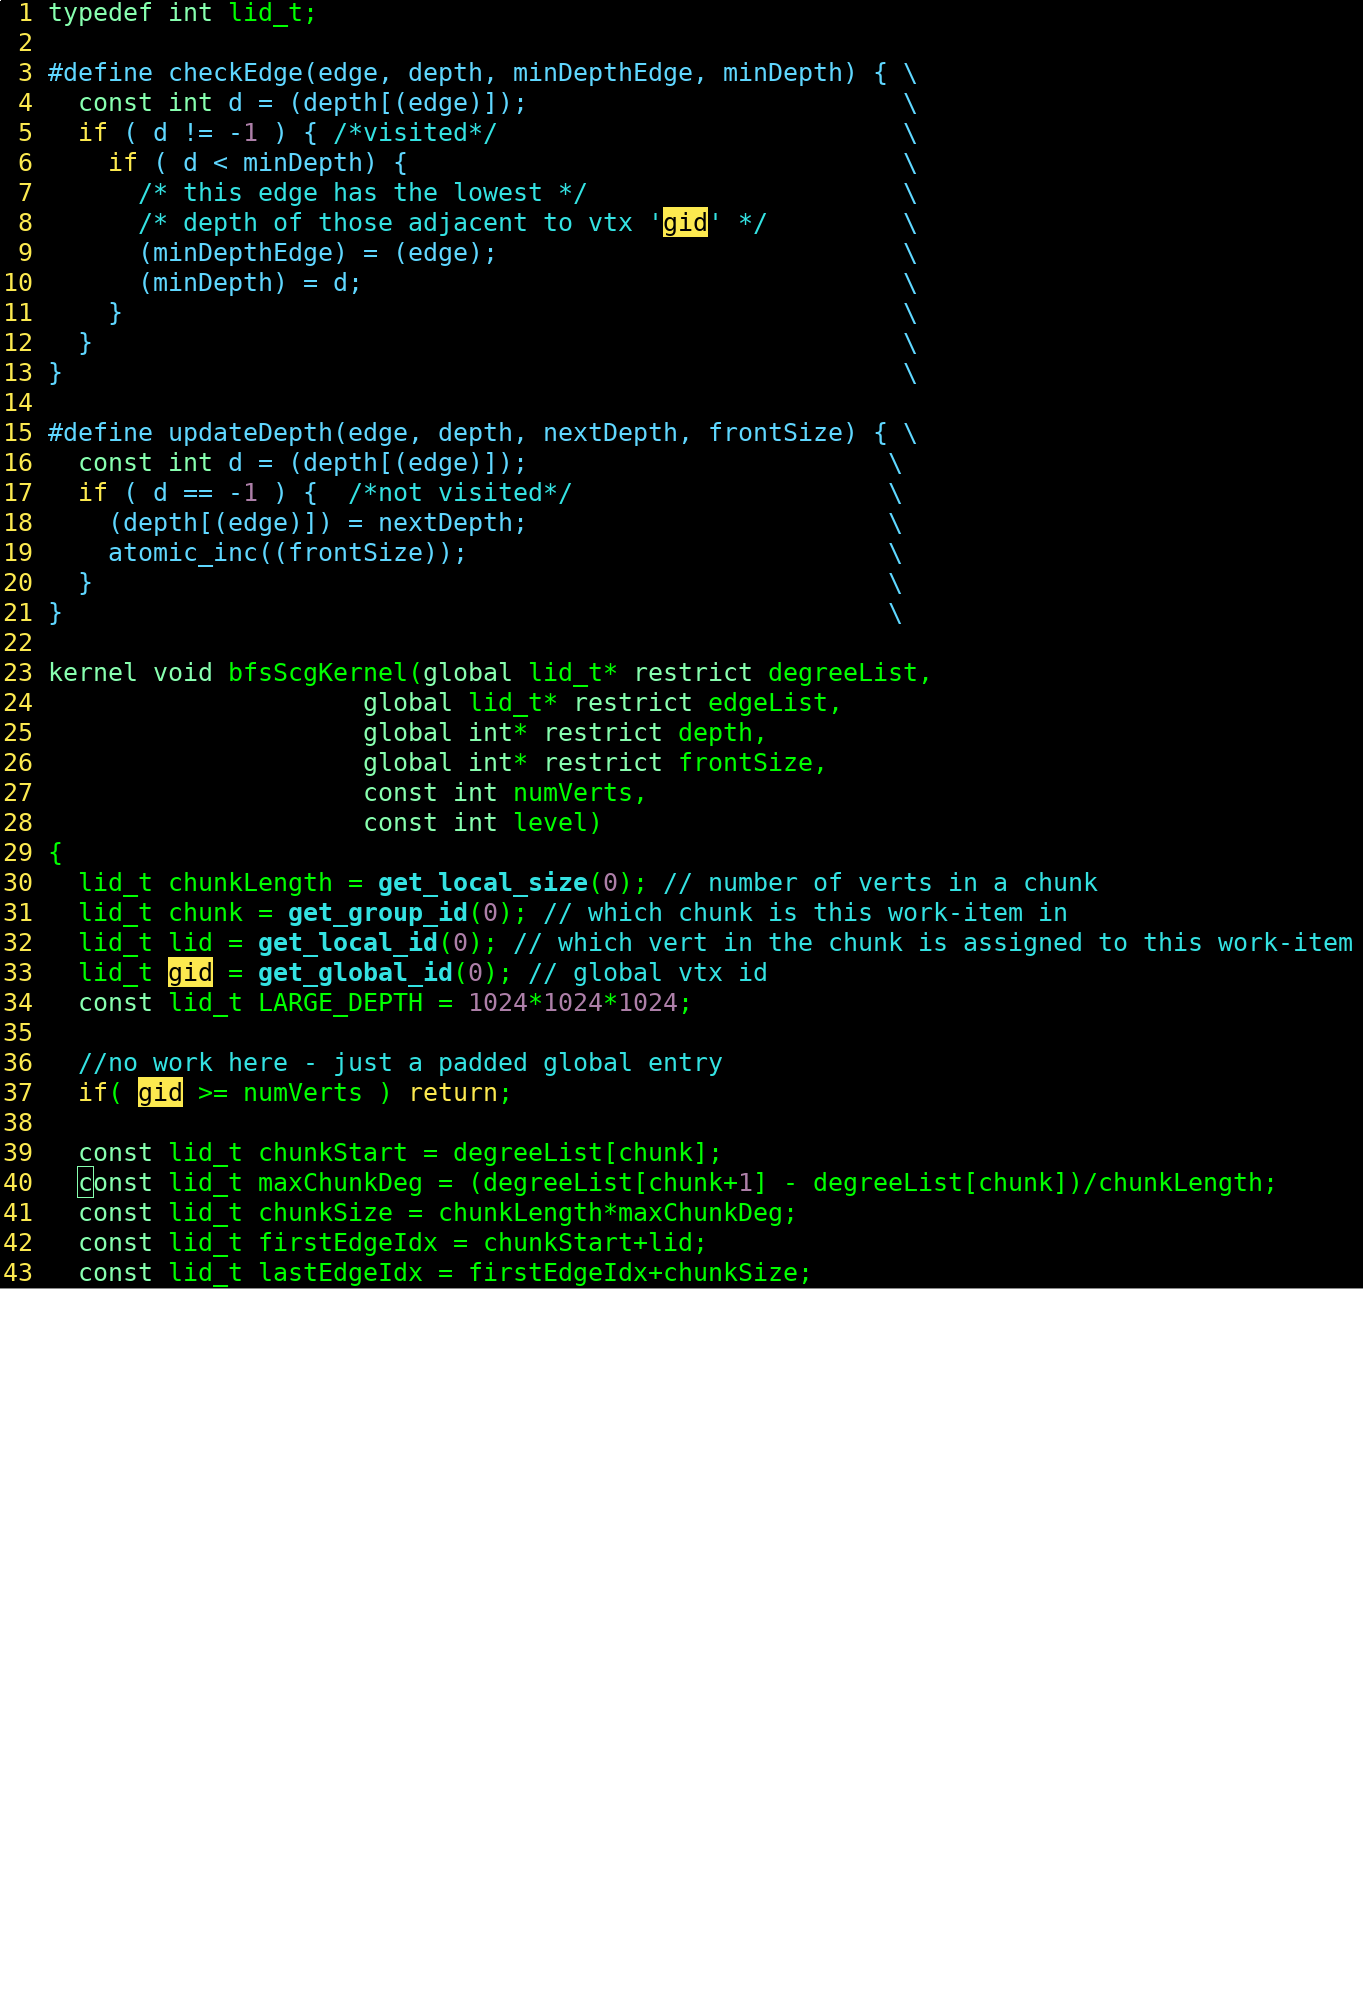
\includegraphics[width=\textwidth]{figures/bfsScgKernelp1.png}
      \end{figure}  
    \end{column}
    \begin{column}{0.5\textwidth}
      \begin{figure}
        \vspace*{-2cm}
        \centering
        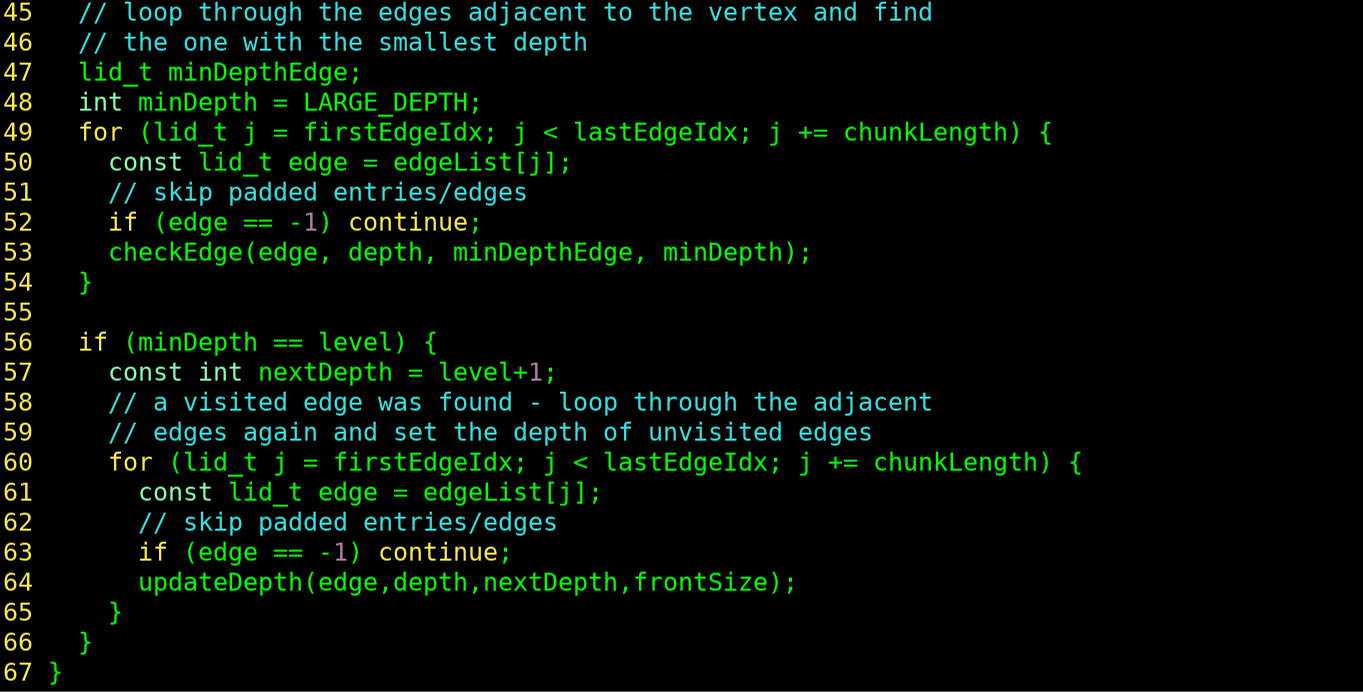
\includegraphics[width=\textwidth]{figures/bfsScgKernelp2.png}
      \end{figure}  
      Loop:
      \begin{figure}
        \centering
        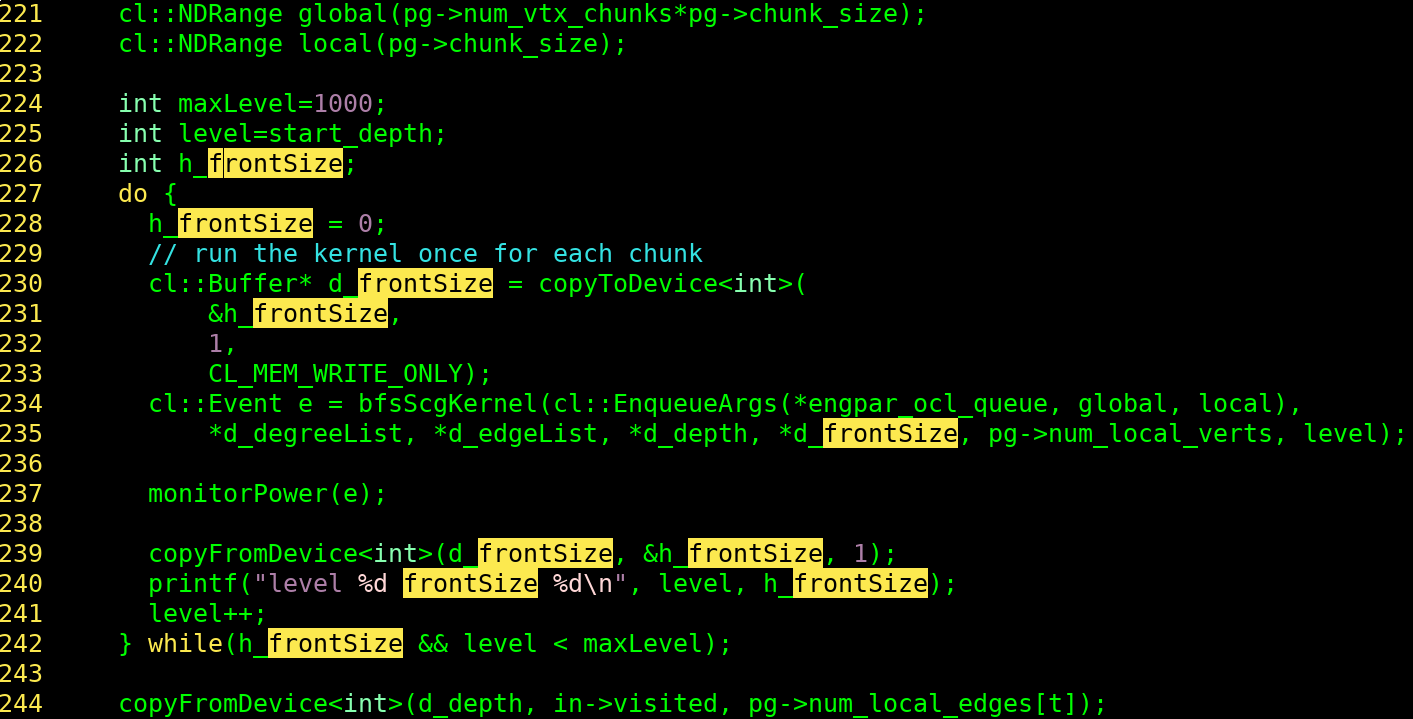
\includegraphics[width=\textwidth]{figures/kernelLoop.png}
      \end{figure}  
    \end{column}
  \end{columns}
\end{frame}


\begin{frame}{Power Consumption scg\_int\_unroll}
  \begin{table}[]
    \centering
    \begin{tabular}{lrrr}
      device & 1080ti               & Arria 10             &               \\
      graph & total power (W)      & total power (W)      & arria10/1080i \\
      67k   & 1.17                 & 0.52                 & 0.45          \\
      190k  & 1.59                 & 1.86                 & 1.17          \\
      400k  & 1.68                 & 4.40                 & 2.61          \\
      890k  & 3.46                 & 13.07                & 3.78          \\
      1.6M  & 5.64                 & 26.48                & 4.69          \\
      13M   & 60.50                & 488.22               & 8.07          \\
      28M   & 151.32               & 1535.60              & 10.15
    \end{tabular}
  \end{table}
  Based on GPU draw of 215W and FPGA draw of 30W\\
  Measured with \texttt{nvidia-smi} and \texttt{aocl\_mmd\_getinfo}
\end{frame}


\begin{frame}{Run time}
  \begin{table}[]
    \small
    \centering
    \begin{tabular}{lrrrr}
      device & i7           & 1080ti               & Arria 10             & i3                   \\
      C &              & 64                   & 64                   & 64                   \\
      graph & push bfs (s) & scg\_int\_unroll (s) & scg\_int\_unroll (s) & scg\_int\_unroll (s) \\
      67k   & 0.011        & 0.005                & 0.017                & 0.013                \\
      190k  & 0.037        & 0.007                & 0.062                & 0.069                \\
      400k  & 0.076        & 0.008                & 0.147                & 0.150                \\
      890k  & 0.169        & 0.016                & 0.436                & 0.530                \\
      1.6M  & 0.292        & 0.026                & 0.883                & 1.196                \\
      13M   & 2.535        & 0.281                & 16.274               & 22.727               \\
      28M   & 5.639        & 0.704                & 51.187               & OOM                 
    \end{tabular}
  \end{table}
  Includes data transfers, but not kernel JIT compilation\\
  The average of three runs is used for the comparison
\end{frame}

\end{document}


